\documentclass[a4paper,11pt]{article}
\author{ 杨旭鹏  \  PB17000234}
\date{2019年秋季}
\title{计算物理A 第十七题}

\usepackage{ctex}
\usepackage{amsmath}
\usepackage{amsfonts}
\usepackage{graphicx}
\usepackage{epstopdf}
\usepackage{lastpage}
\usepackage{hyperref}
\usepackage{listings}
\RequirePackage{xcolor}
\usepackage{appendix}
\usepackage{caption2}
\usepackage{subfigure}
\usepackage{float}
\usepackage{verbatim}
\usepackage{fancybox}
\usepackage{geometry}
\geometry{left=3cm,right=3cm,top=2.5cm,bottom=2.5cm}
\makeatletter\def\@captype{table}\makeatother
\usepackage{tikz}
\usetikzlibrary{shapes,arrows}
\tikzstyle{startstop} = [rectangle,rounded corners, minimum width=3cm,minimum height=1cm,text centered, draw=black,fill=red!30]
\tikzstyle{io} = [trapezium, trapezium left angle = 70,trapezium right angle=110,minimum width=3cm,minimum height=1cm,text centered,draw=black,fill=blue!30]
\tikzstyle{process} = [rectangle,minimum width=4cm,minimum height=1cm,text centered, text width=4cm, draw=black,fill=orange!30]
\tikzstyle{decision} = [diamond,minimum width=3cm,minimum height=1cm,text centered,draw=black,fill=green!30]
\tikzstyle{arrow} = [thick,->,>=stealth]


\definecolor{dkgreen}{rgb}{0,0.6,0}
\definecolor{gray}{rgb}{0.5,0.5,0.5}
\definecolor{mauve}{rgb}{0.58,0,0.82}

\lstset{
  frame=tb,
  aboveskip=3mm,
  belowskip=3mm,
  showstringspaces=false,
  columns=flexible,
  framerule=1pt,
  rulecolor=\color{gray!35},
  backgroundcolor=\color{gray!5},
  basicstyle={\small\ttfamily},
  numbers=left,
  numberstyle=\tiny\color{gray},
  keywordstyle=\color{blue},
  commentstyle=\color{dkgreen},
  stringstyle=\color{mauve},
  breaklines=true,
  breakatwhitespace=true,
  tabsize=3,            
  }



\begin{document}
\maketitle
\tableofcontents

\section{题目描述}
考虑一维经典粒子组成的理想气体,由于无相互作用,各粒子的能量不依赖于其位置,只需考虑它的动能,因此体系的构型即是各粒子速度坐标值的集合。给定粒子的质量、初始速度、总粒子数、总能、demon能,模拟足够多步后达到平衡时的粒子速度分布。微正则系综中没有定义温度,其数值由$\frac{1}{2}kT = \frac{1}{2}m \left < v^{2} \right> $给出,求平衡时的温度值。



\section{微正则系综 Monte Carlo 模拟方法}

设初始情况一维粒子速度$V_{i}$在$[-1,1]$间均与分布,质量$m = 1$,Demon能$E_{d} = 0$。设粒子总数为$n$,能量每步改变范围为$(-\Delta,\Delta)$。

\begin{tikzpicture}[node distance=2.5cm]
\node (start) [startstop] {$V_{i}$在$[-1,1]$间均与分布,$E_{d} = 0$};
\node (gen1) [process,below of=start] {在$[1,n]$均匀抽取整数$i$};
\node (gen11) [process,below of= gen1] {产生在$(-\Delta,\Delta)$均匀分布的随机数$\delta$};
\node (dE) [process,below of=gen11]{计算能量差 \\ $\Delta E  = \frac{1}{2} m[ (v_{i} + \delta)^{2} -v_{i}^{2} ]$};
\node (decision1) [decision,below of = dE ,yshift=-0.5cm] {$\Delta E \leq 0$};
\node (233) [process,left of = decision1,xshift = -2cm]{进行下一轮计算};
\node (decision2) [decision,right of =decision1,xshift=2.5cm] {$E_{d}\geq \Delta E$};
\node (value) [process,below of=decision1,yshift=-0.5cm] {$v_{i} = v_{i} + \delta  $ \\ $ E_{d} = E_{d} - \Delta E$};
\node (decision3) [decision,below of = value ,yshift=-0.5cm] {循环次数足够};
\node (end) [startstop, below of = decision3] {程序结束};


\draw [arrow] (start) -- (gen1);
\draw [arrow] (gen1) -- (gen11);
\draw [arrow] (gen11) -- (dE);
\draw [arrow] (dE) -- (decision1);
\draw [arrow] (decision1) -- node[anchor=south] {no} (decision2);
\draw [arrow] (decision1) -- node[anchor=west] {yes} (value);
\draw [arrow] (decision2) |-  node[anchor=south] {no}(gen1);
\draw [arrow] (decision2) |-  node[anchor=west] {yes}(value);
\draw [arrow] (value) -- (decision3);
\draw [arrow] (decision3) -- node[anchor=west] {yes} (end);
\draw [arrow] (decision3) -| node[anchor=north] {no} (233);
\draw [arrow] (233) |- (gen1);	

\end{tikzpicture}

算法流程图如上所示。

\section{理论推导}
为简化计算,规定$T = m \left < v^{2} \right>$,则可推知:
\begin{equation}
	T = \frac{\int_{-1}^{1} v^{2} dv}{2} = \frac{1}{3} \approx 0.33333
\end{equation}

而平衡态理想气体速度分布满足高斯分布:
\begin{equation}
	p(v) = \sqrt{\frac{1}{2\pi T}} e^{-\frac{v^{2}}{2T}} = \sqrt{\frac{3}{2\pi}} e^{-\frac{3}{2}v^{2}}
\end{equation}

而对于$E_{d}$,根据计算物理讲义上的内容,其满足Bolzman分布:
\begin{equation}
	p(E_{d}) = \frac{1}{T} e^{-\frac{E_{d}}{T}} = 3e^{-3E_{d}}
\end{equation}

\section{程序使用方法}
此程序设计为参数在程序代码中直接赋值形式,每次需在程序源码中进行参数调整,进而编译运行,以简化每次输入的过程(重复运行时不用在此输入)。需要调整的参数包括main函数中的粒子总个数$n$,进行模拟总步数$N$,计算粒子温度$T$及demon能$E_{d}$的步数间隔,每一个粒子每一次速度该变量参数$\Delta$。调整完参数后,编译运行,程序会自动输出不同步数对应的$T,E_{d}$,模拟最后一步时粒子的速度分布至不同文件。

\newpage
\section{程序结果与讨论}
\subsection{粒子平衡时的温度}
当设定粒子总数$n=10^{4}$,模拟总步数$N=10^{7}$,每计算$1000$步统计粒子的温度$T$和$E_{d}$时,得到结果:

\begin{figure}[!htbp]   
\centering     
\subfigure[粒子温度统计结果]{
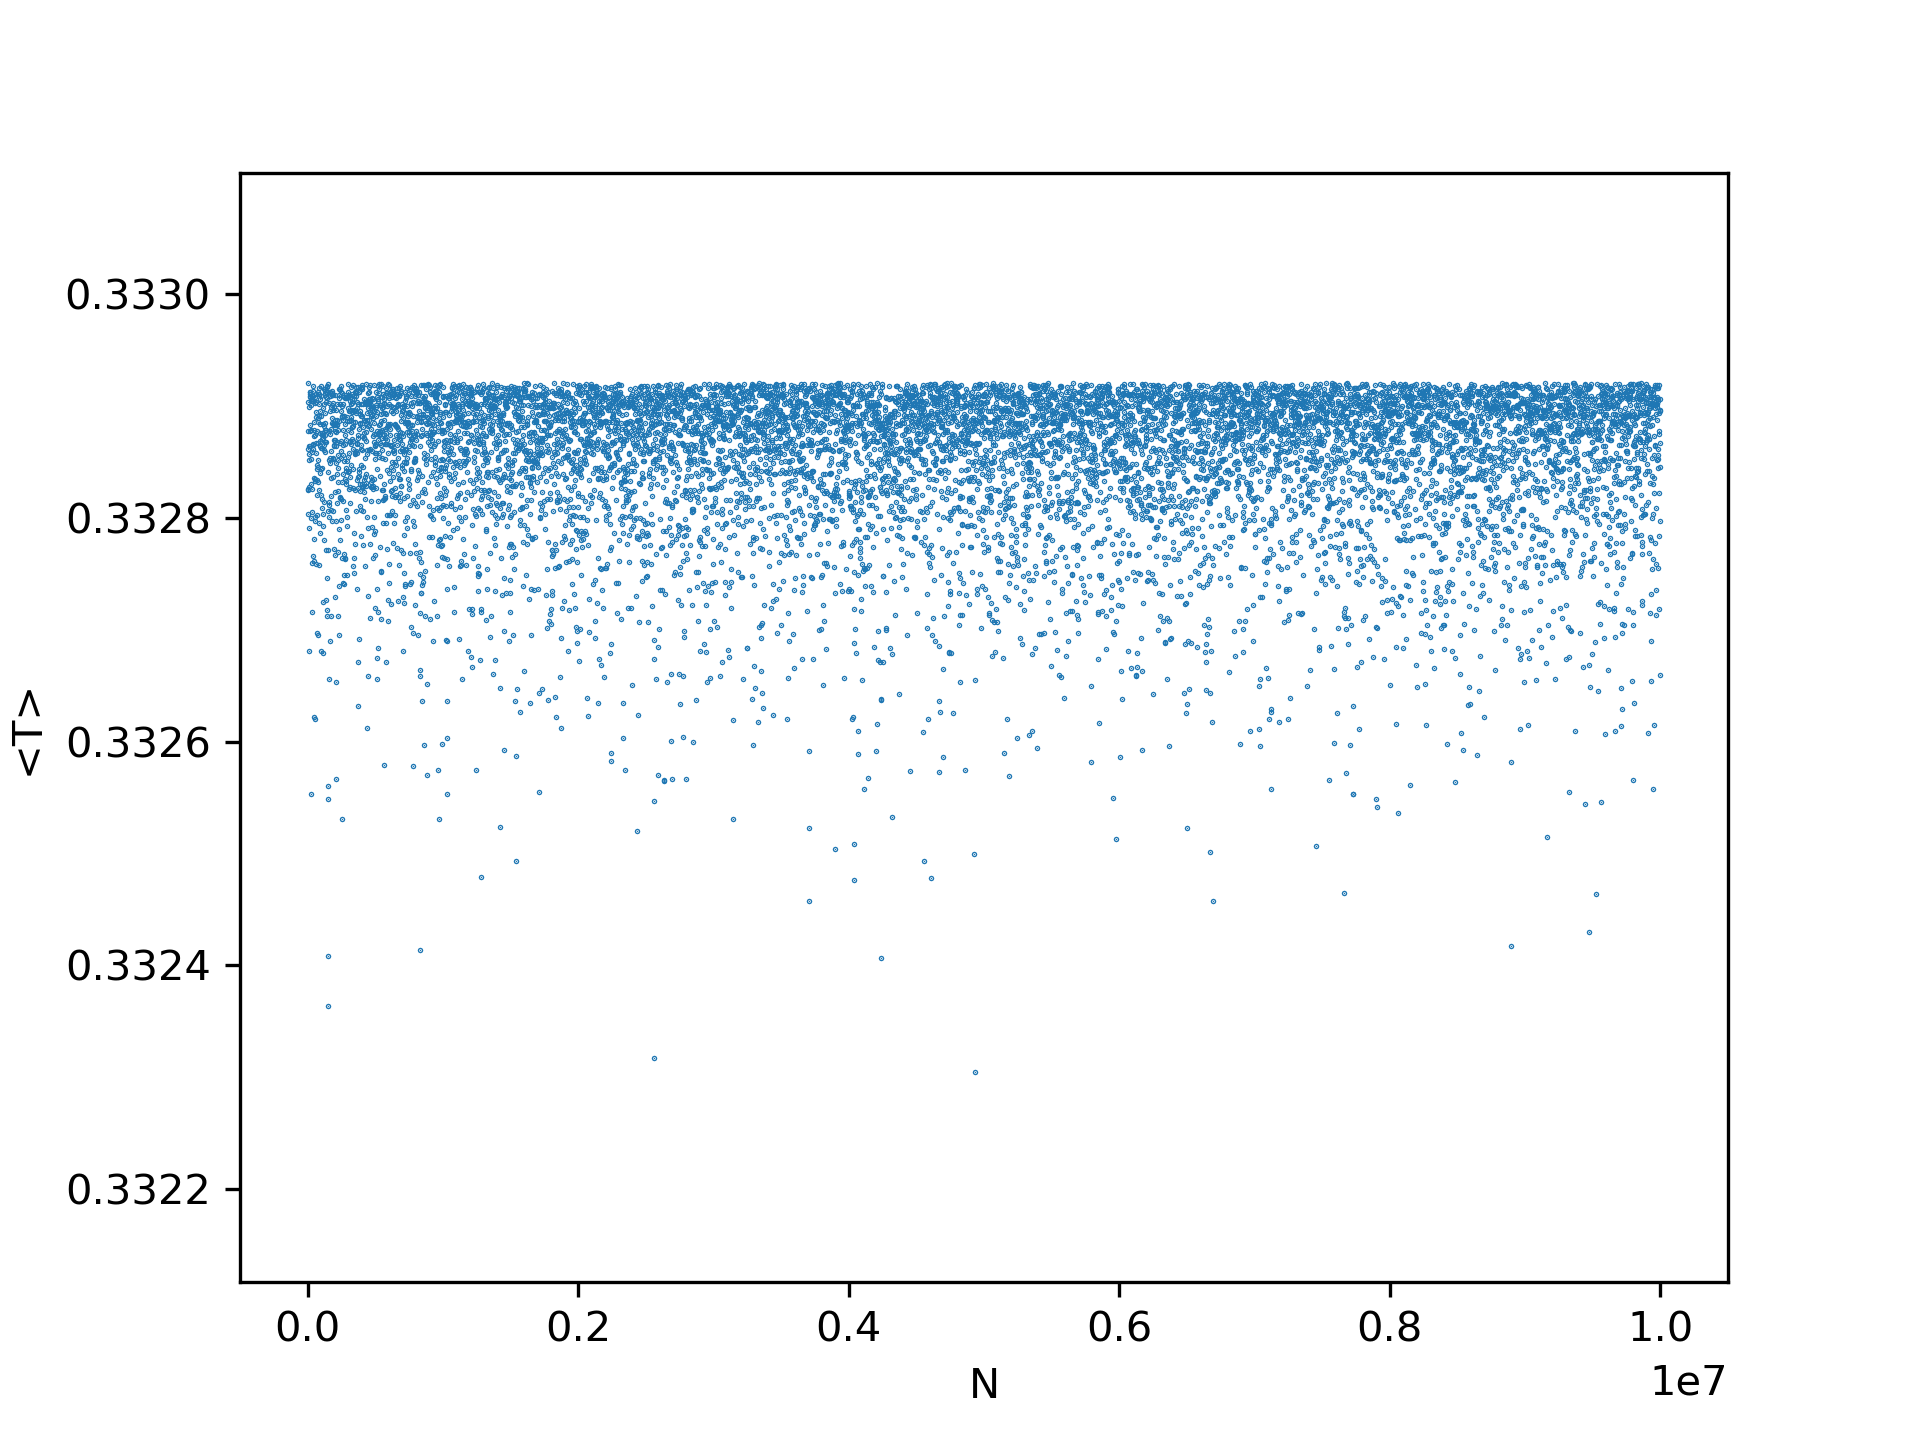
\includegraphics[bb= 0 0 460.8 345.6,width=7cm] {0.1-104-107-T.png}
}
\subfigure[$E_{d}$统计结果]{
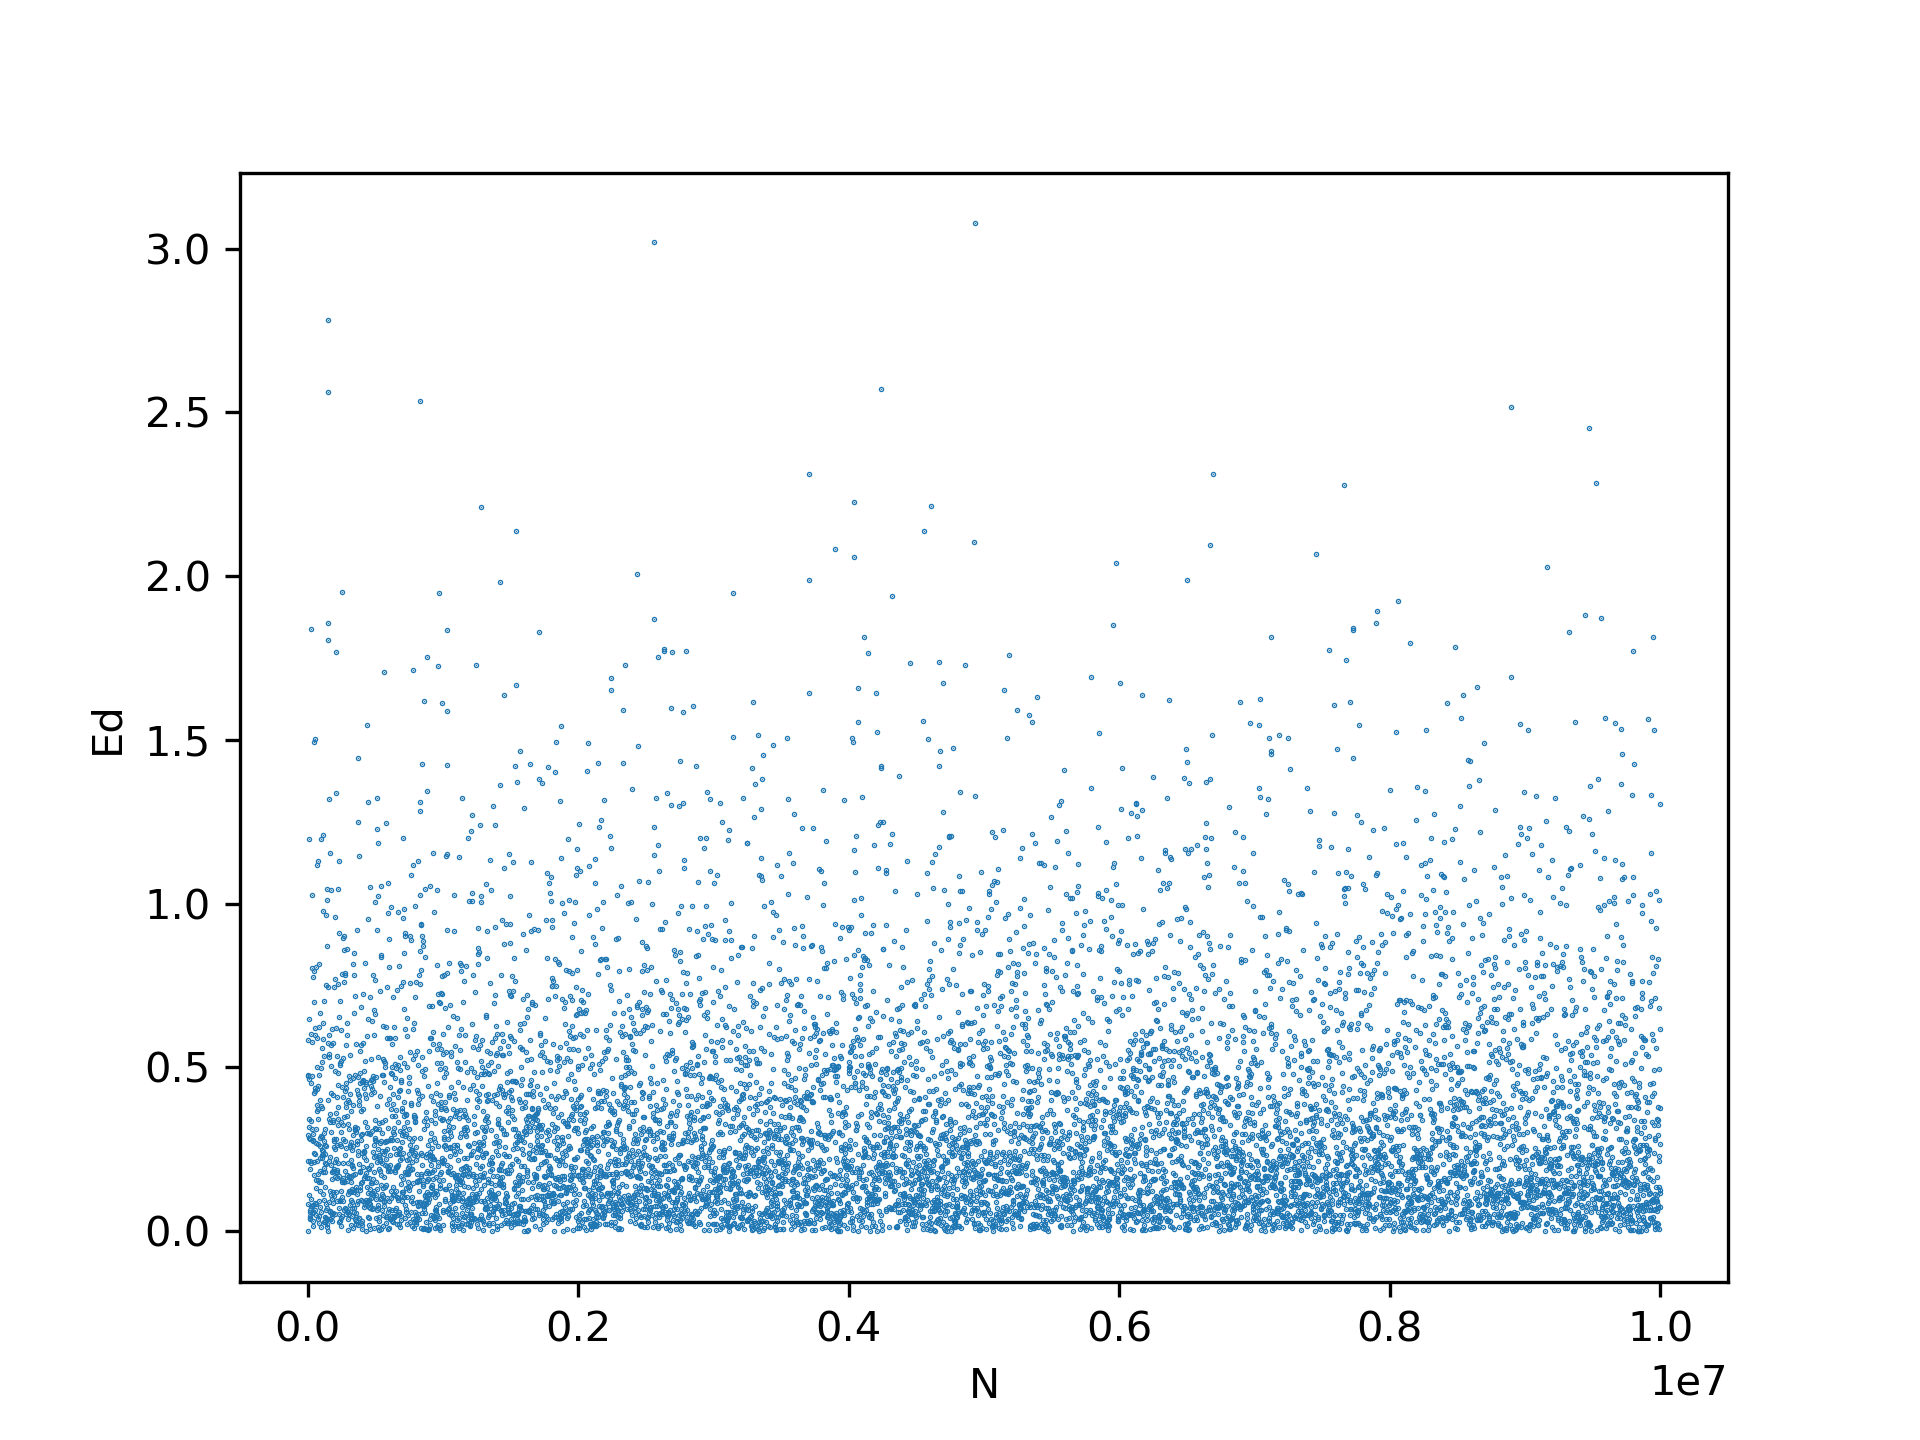
\includegraphics[bb= 0 0 460.8 345.6,width=7cm] {0.1-104-107-Ed.png}
}       
\subfigure[粒子速度$v$的最终分布]{
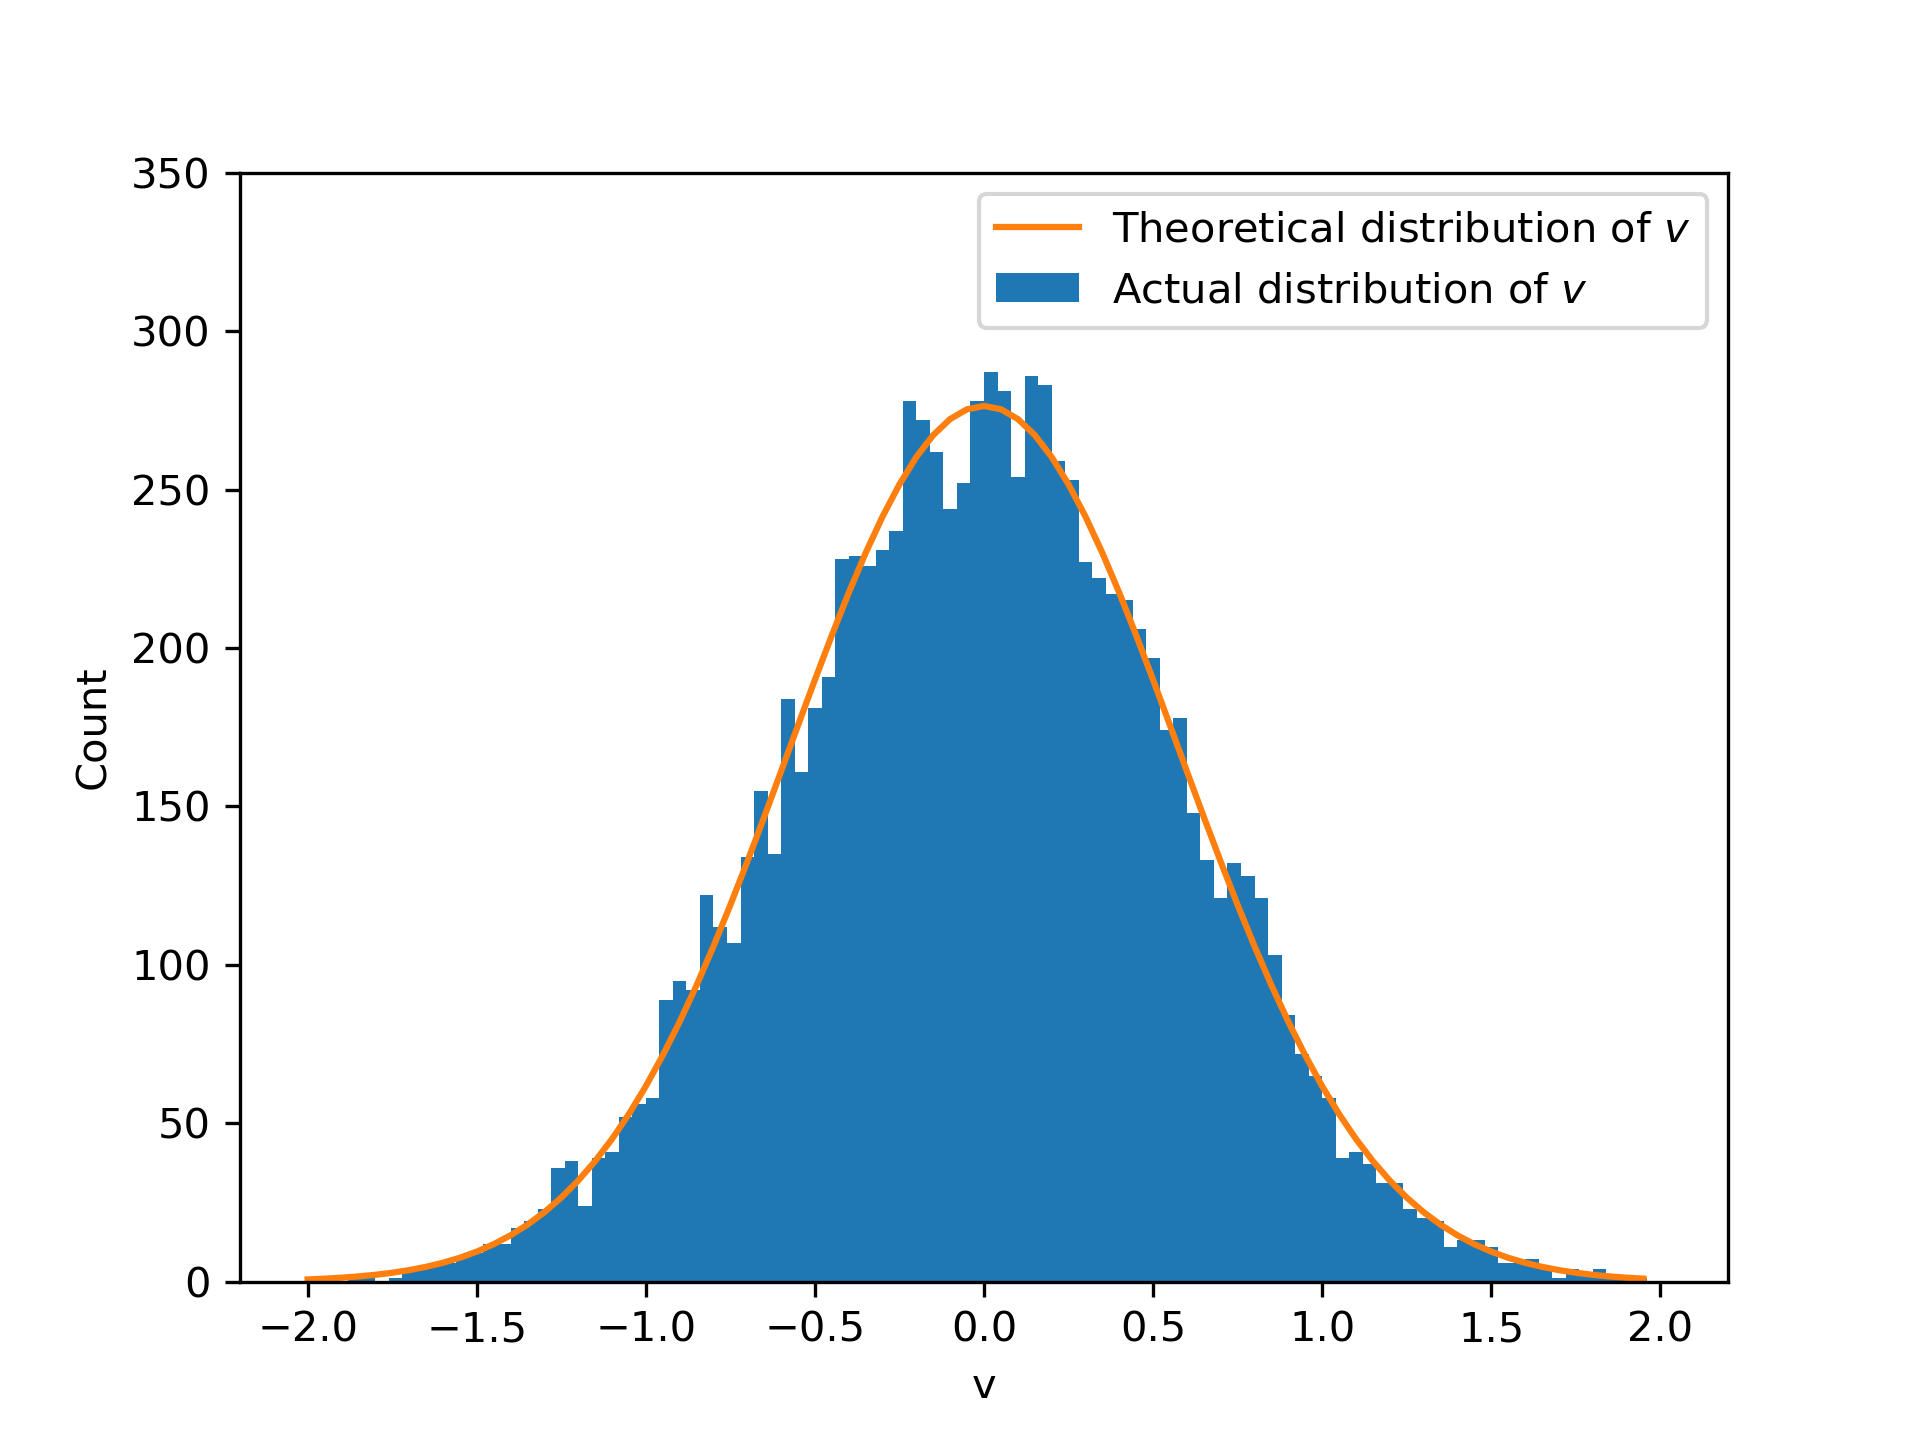
\includegraphics[bb= 0 0 460.8 345.6,width=7cm] {0.1-104-107-v.png}
}   
\subfigure[$E_{d}$的分布]{
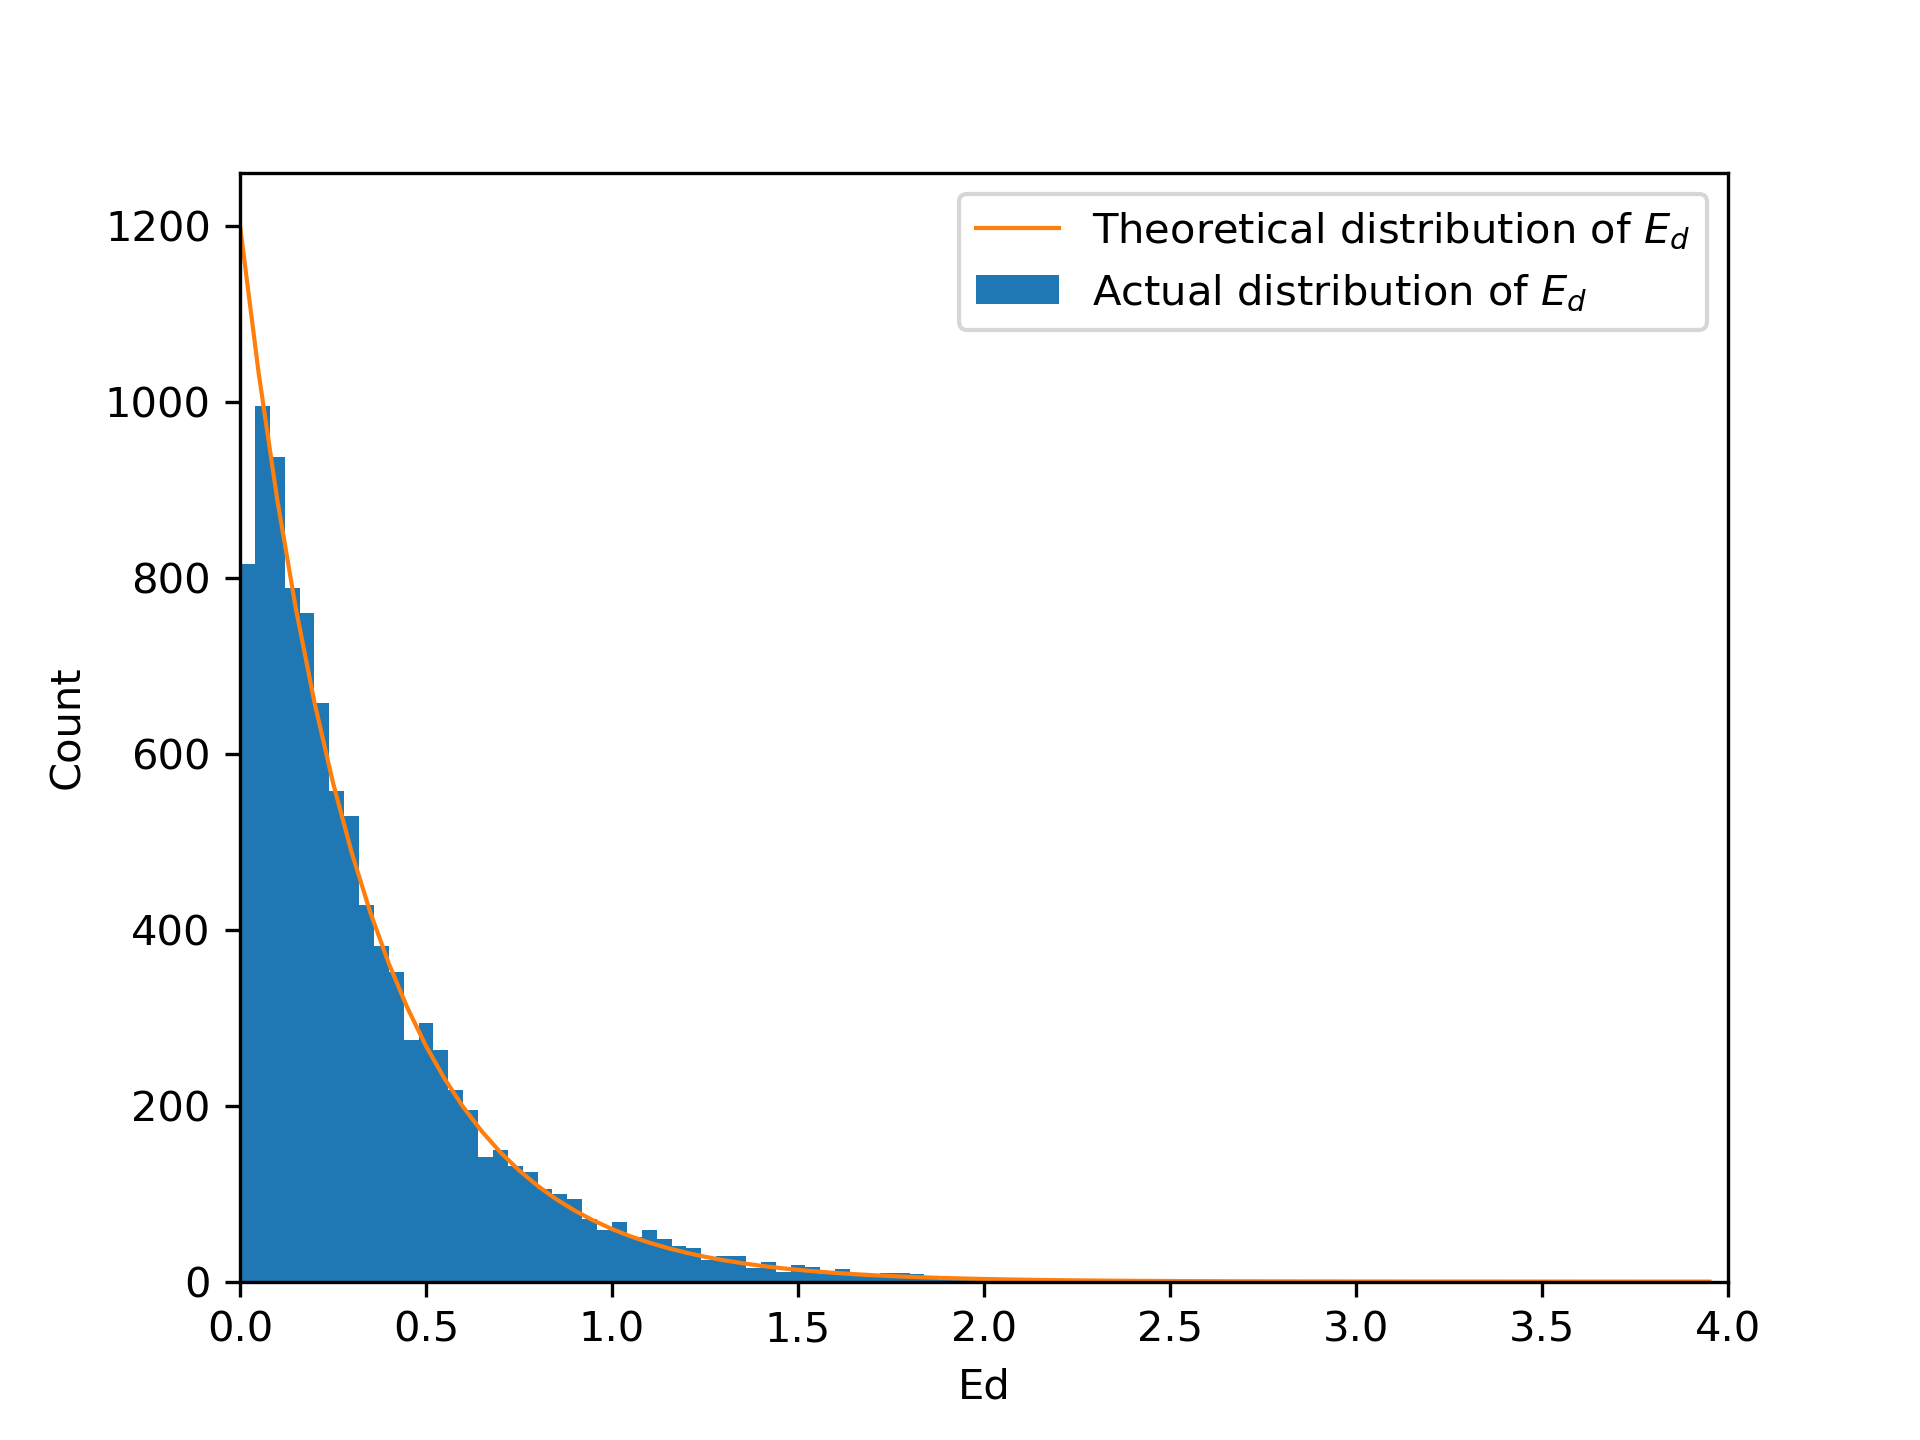
\includegraphics[bb= 0 0 460.8 345.6,width=7cm] {0.1-104-107-Ed-2.png}
}                             
\caption{$\Delta = 0.1$,$n=10^{4}$,$N=10^{7}$,每计算$1000$步统计$T,E_{d}$的结果}      
\end{figure}

其中的理论概率分布均为归一化概率密度函数$p$乘以统计区间长度和总统计个数得到的理论频率曲线。可以看出,粒子的温度基本稳定在$0.332921$,与理论值$\frac{1}{3}$基本一致,差别在于一开始初始化速度时存在统计涨落。而粒子的温度随步数变化幅度较小,基本满足微正则系综的要求。从粒子模拟最后的速度分布看出与理论高斯分布比较接近,若提高粒子总数,猜测能够与理论分布更加接近,但这样会增大计算量。而$E_{d}$的统计分布与理论的Bolzman分布除了在$0$附近也拟合的比较好,这样的结果可能来自于Bolzman$0$附近导数较大,变化比较剧烈,猜测若减小速度改变的步长范围会使$E_{d}$的统计分布更加接近理论分布,但是同样的必须提高计算总步数,才可能使系统达到平衡态,而这样会增加计算量。则可以近似认为模拟步数$N=10^{7}$时系统达到平衡态。达到题目要求。


\subsection{参数对于结果的影响}
若调整速度改变步长参数$\Delta = 1$,得到:

\begin{figure}[!htbp]   
\centering     
\subfigure[粒子温度统计结果]{
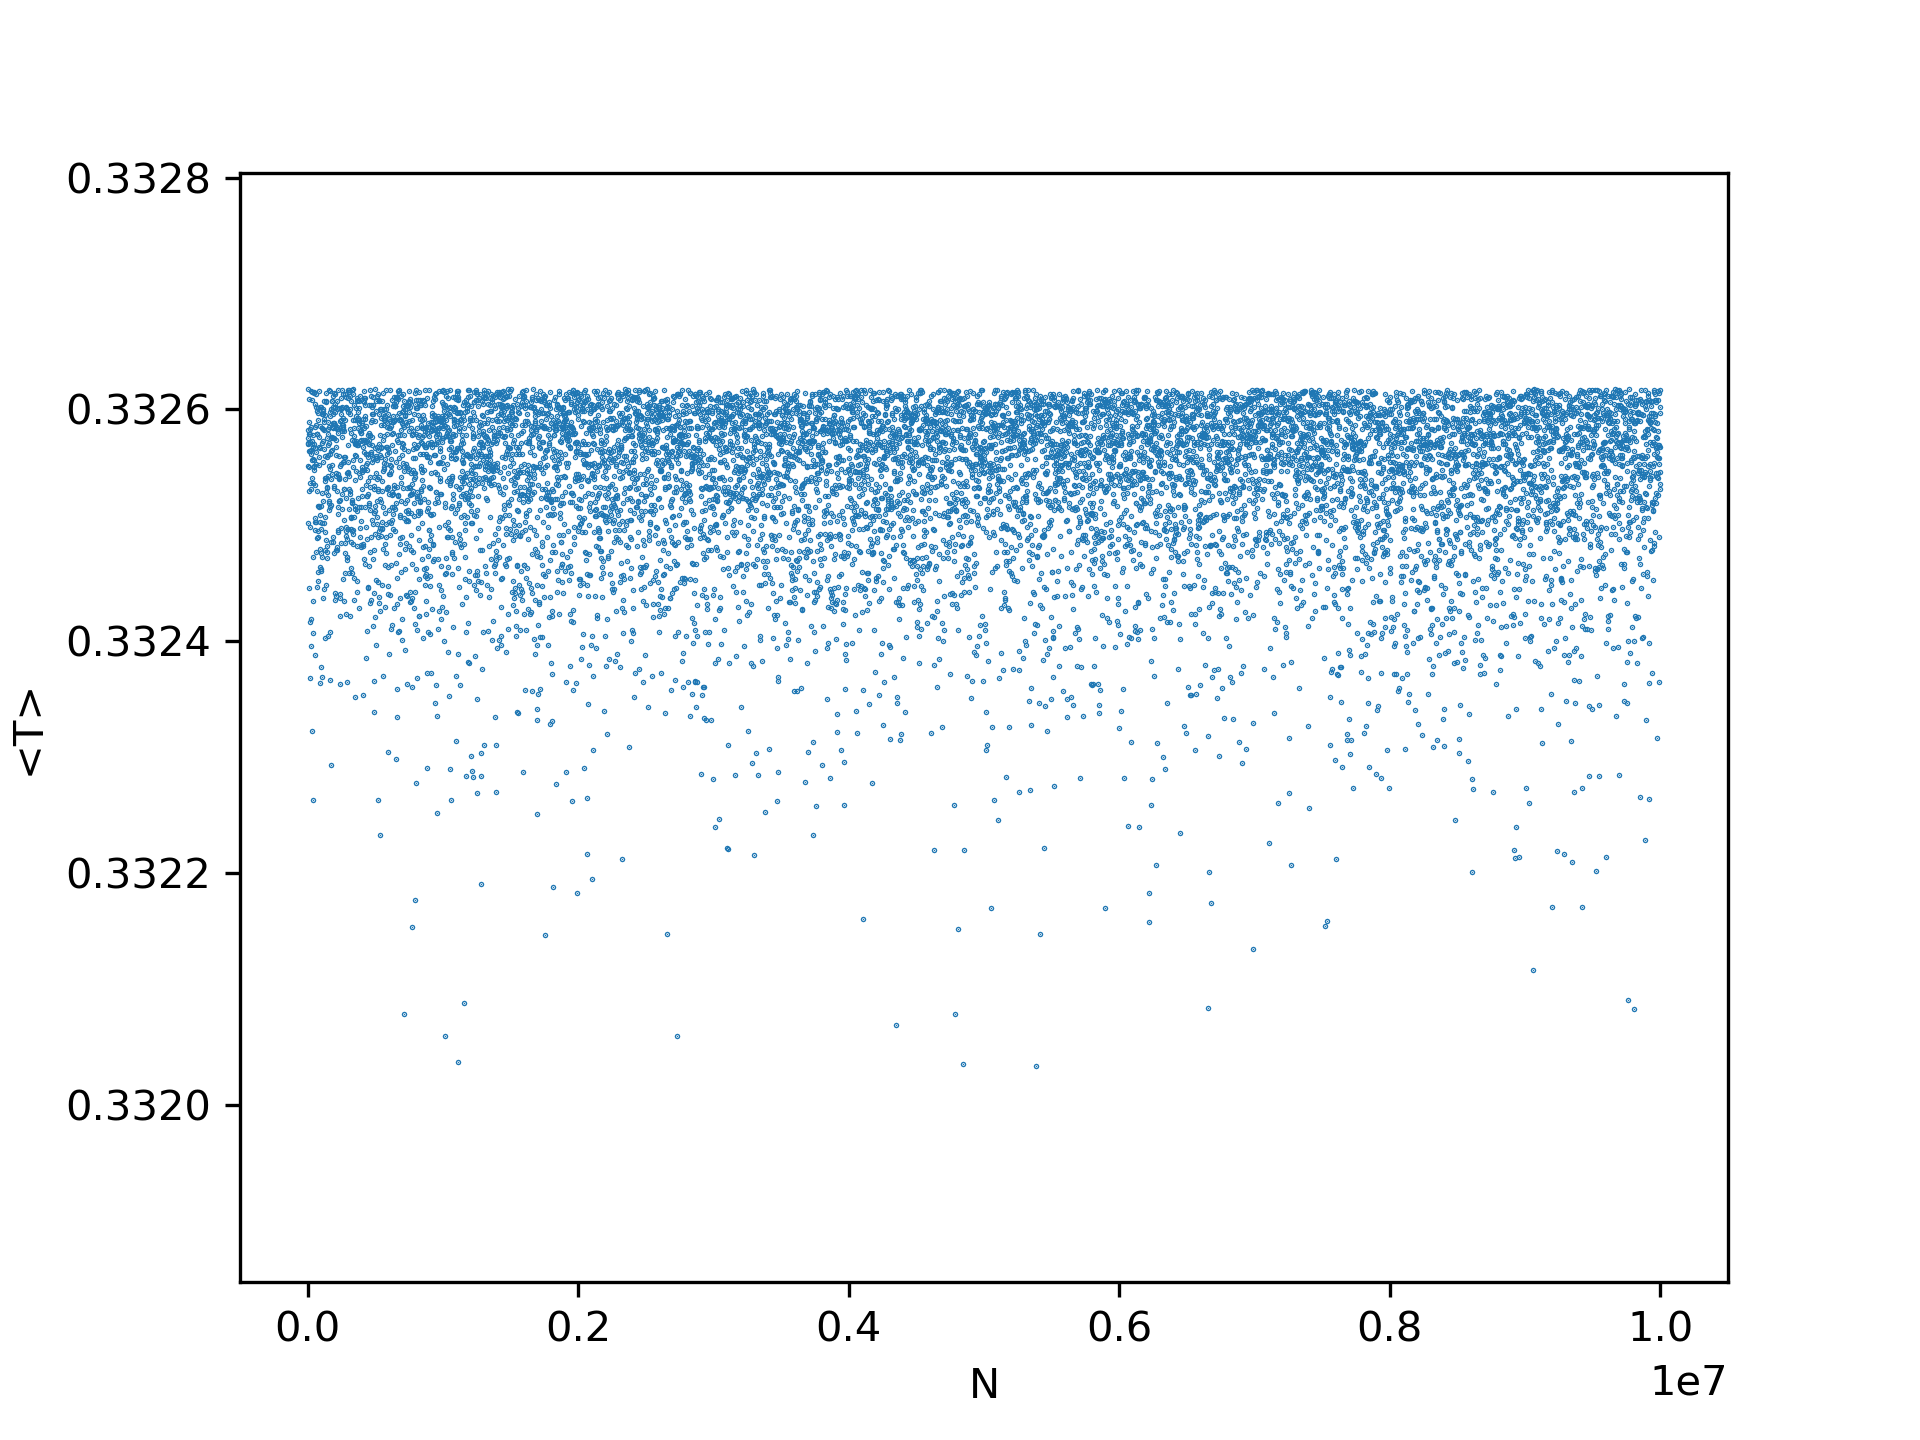
\includegraphics[bb= 0 0 460.8 345.6,width=7cm] {1-104-107-T.png}
}
\subfigure[$E_{d}$统计结果]{
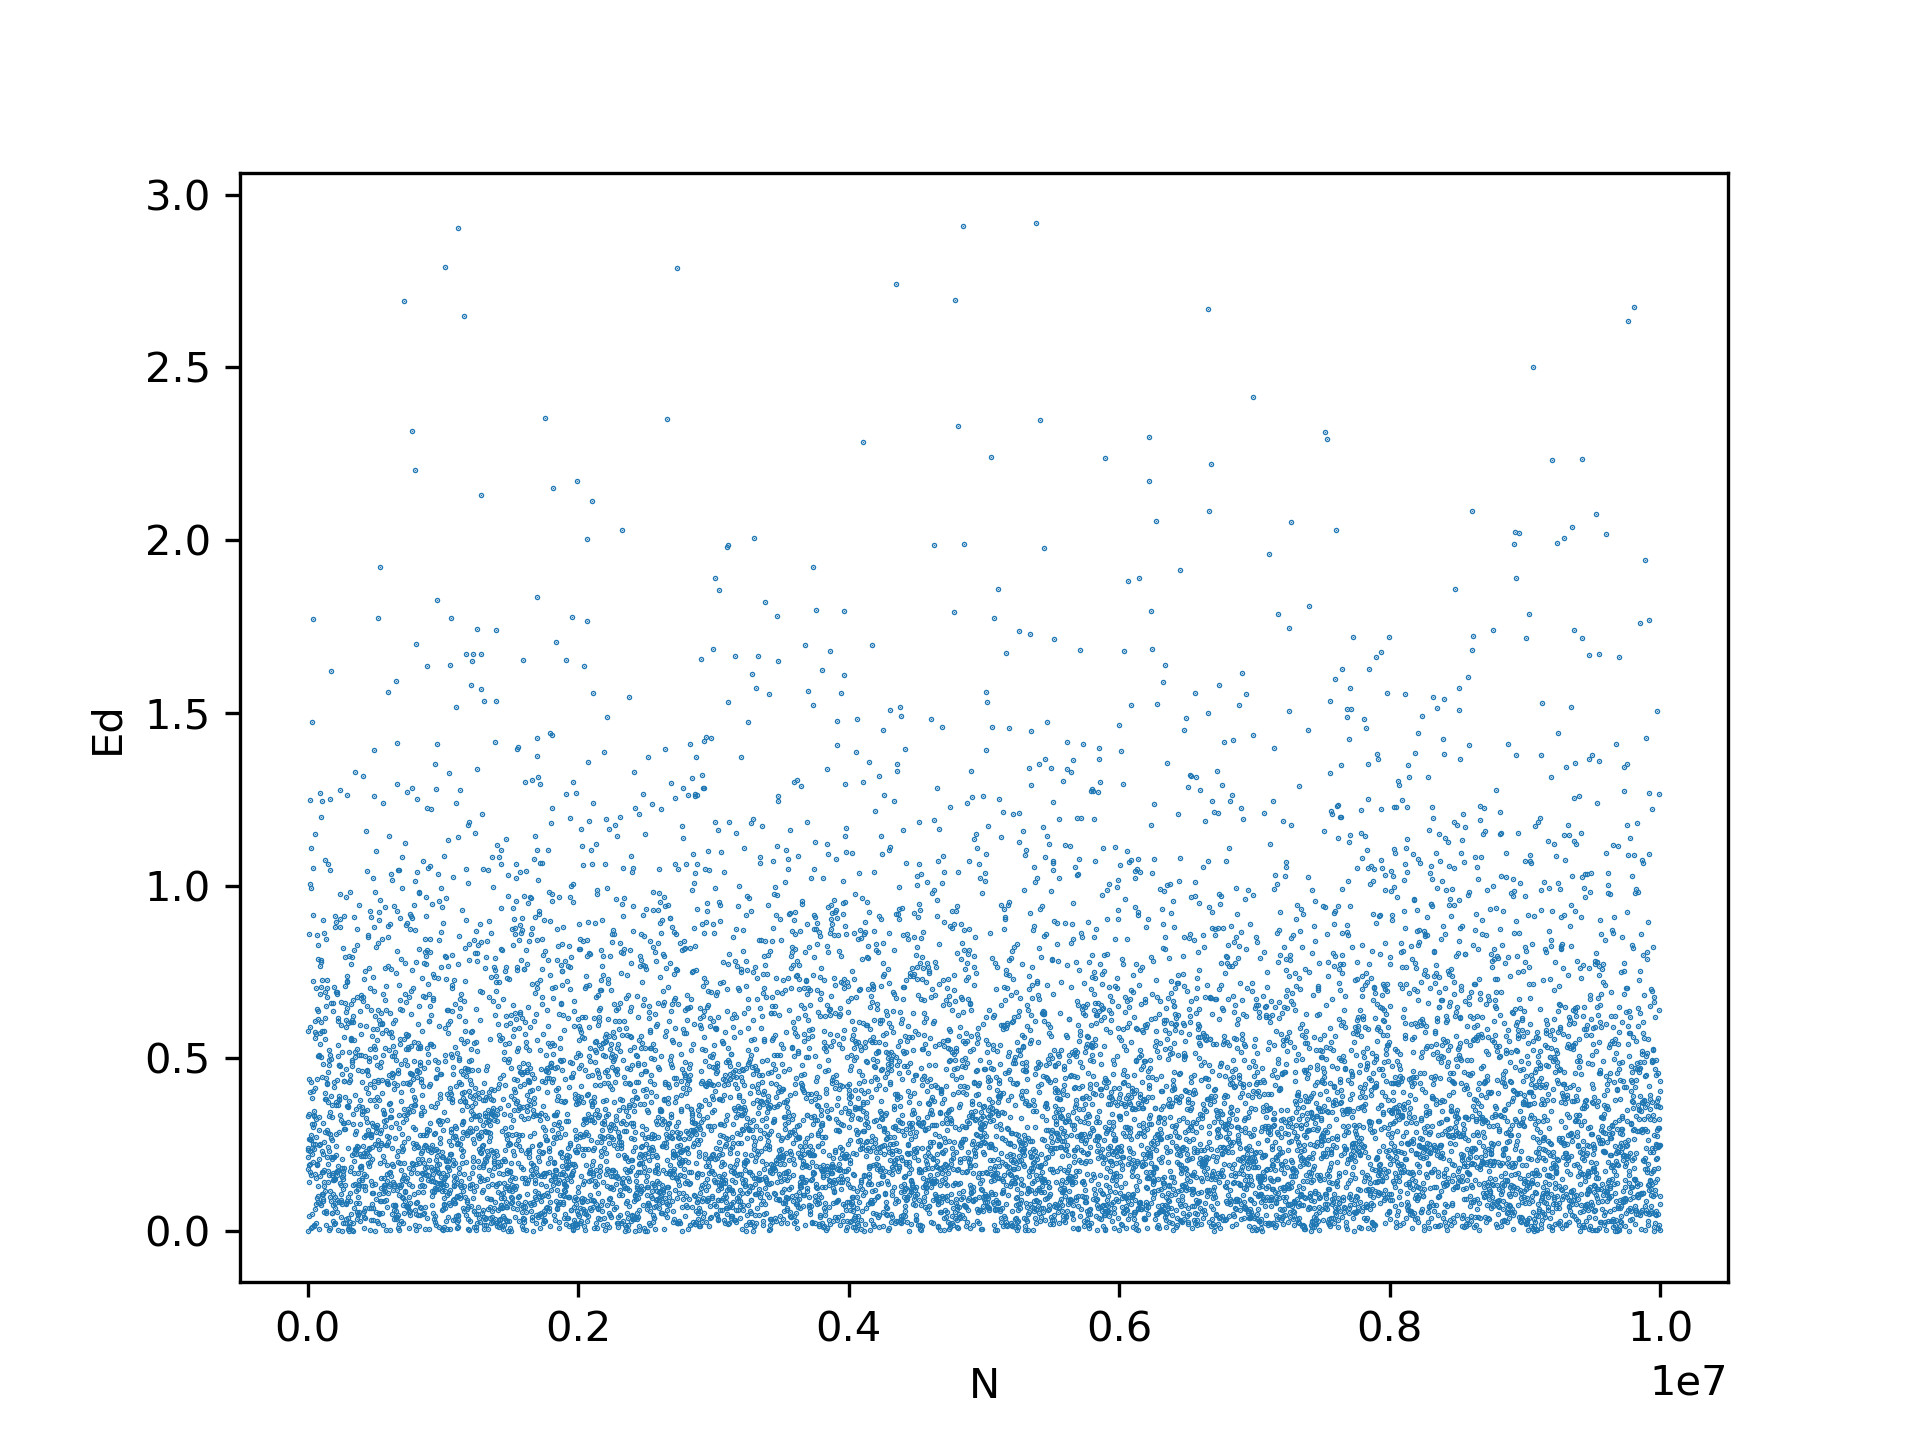
\includegraphics[bb= 0 0 460.8 345.6,width=7cm] {1-104-107-Ed.png}
}       
\subfigure[粒子速度$v$的最终分布]{
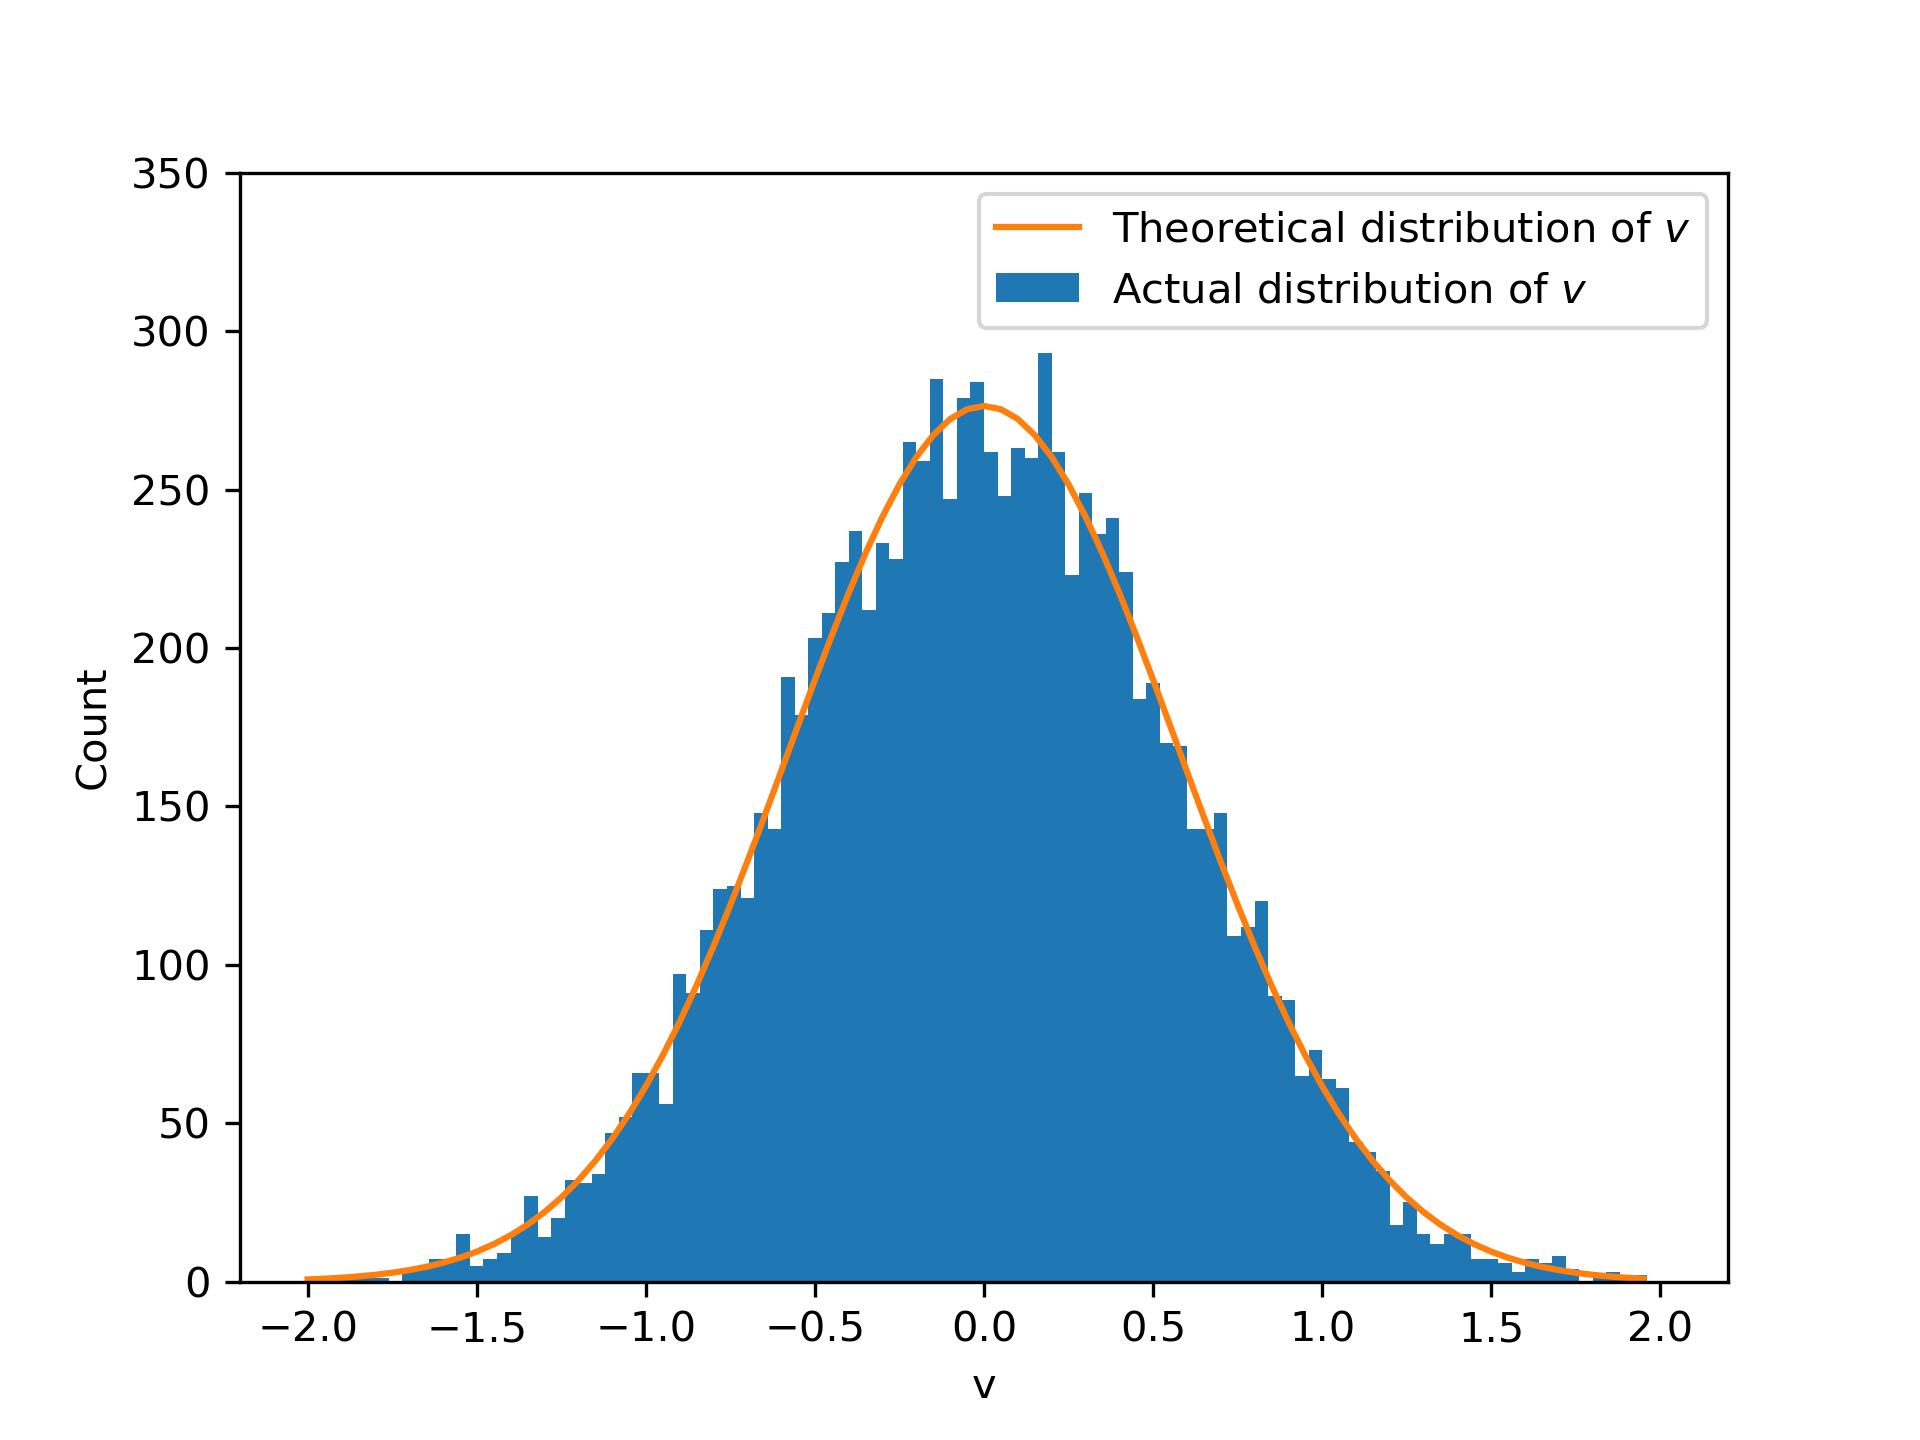
\includegraphics[bb= 0 0 460.8 345.6,width=7cm] {1-104-107-v.png}
}   
\subfigure[$E_{d}$的分布]{
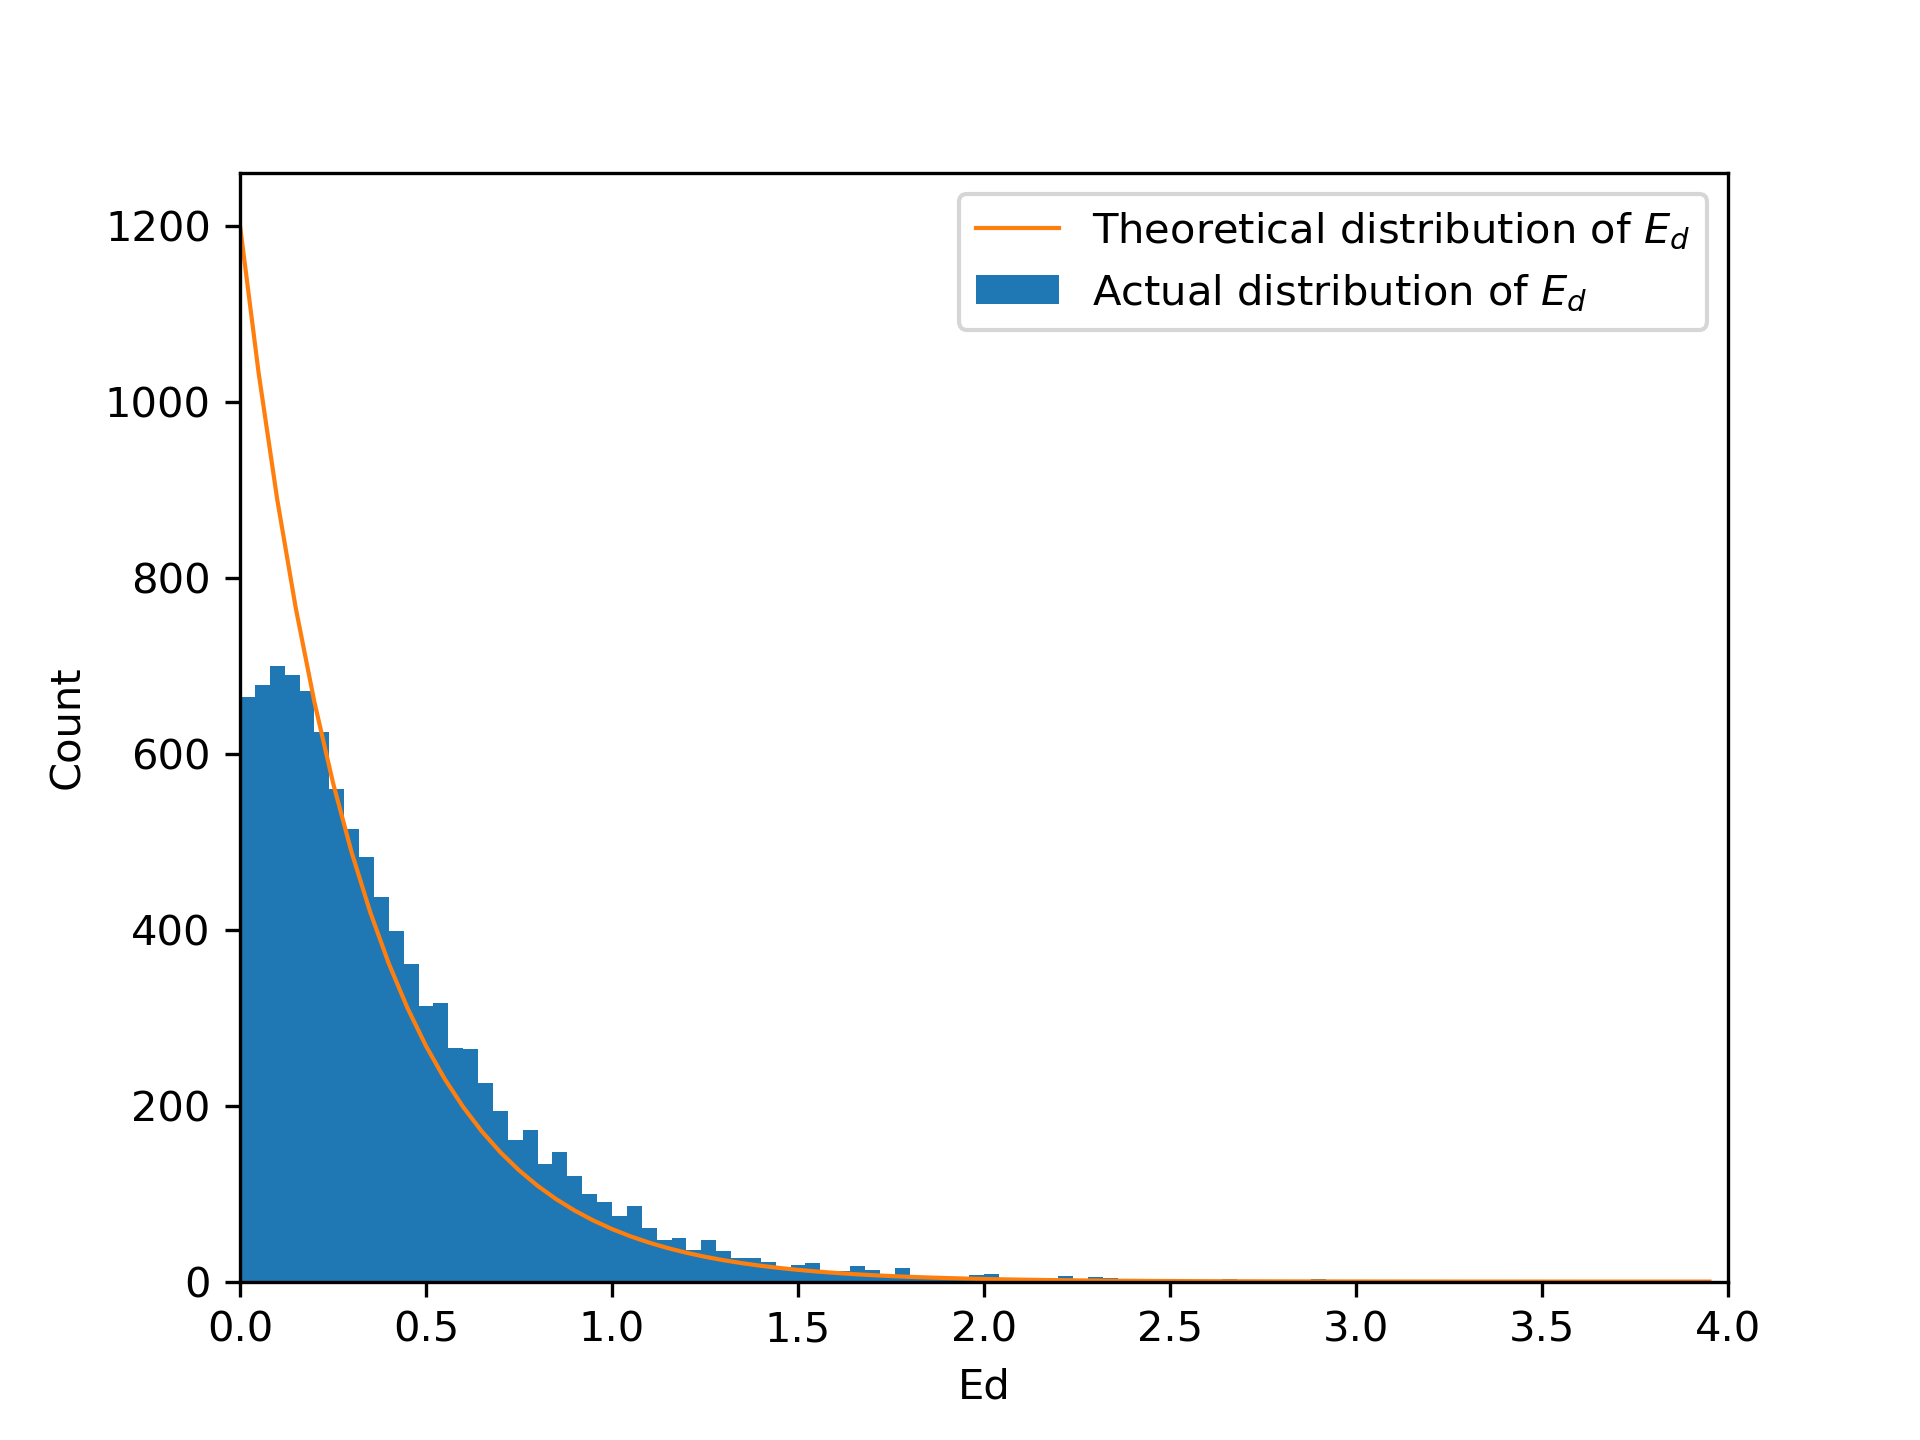
\includegraphics[bb= 0 0 460.8 345.6,width=7cm] {1-104-107-Ed-2.png}
}                             
\caption{$\Delta = 1$,$n=10^{4}$,$N=10^{7}$,每计算$1000$步统计$T,E_{d}$的结果}      
\end{figure}

可以看出步长的变化会导致$E_{d}$的统计分布变化。猜测速度变化步长约小,$E_{d}$更加接近理论分布。因为速度变化步长越大,会迫使本来在0附近的$Ed$下一步变化到离0距离更远的地方,偏离理论分布。

为此,继续调整参数$\Delta = 0.01$,得到:

\begin{figure}[!htbp]   
\centering     
\subfigure[粒子温度统计结果]{
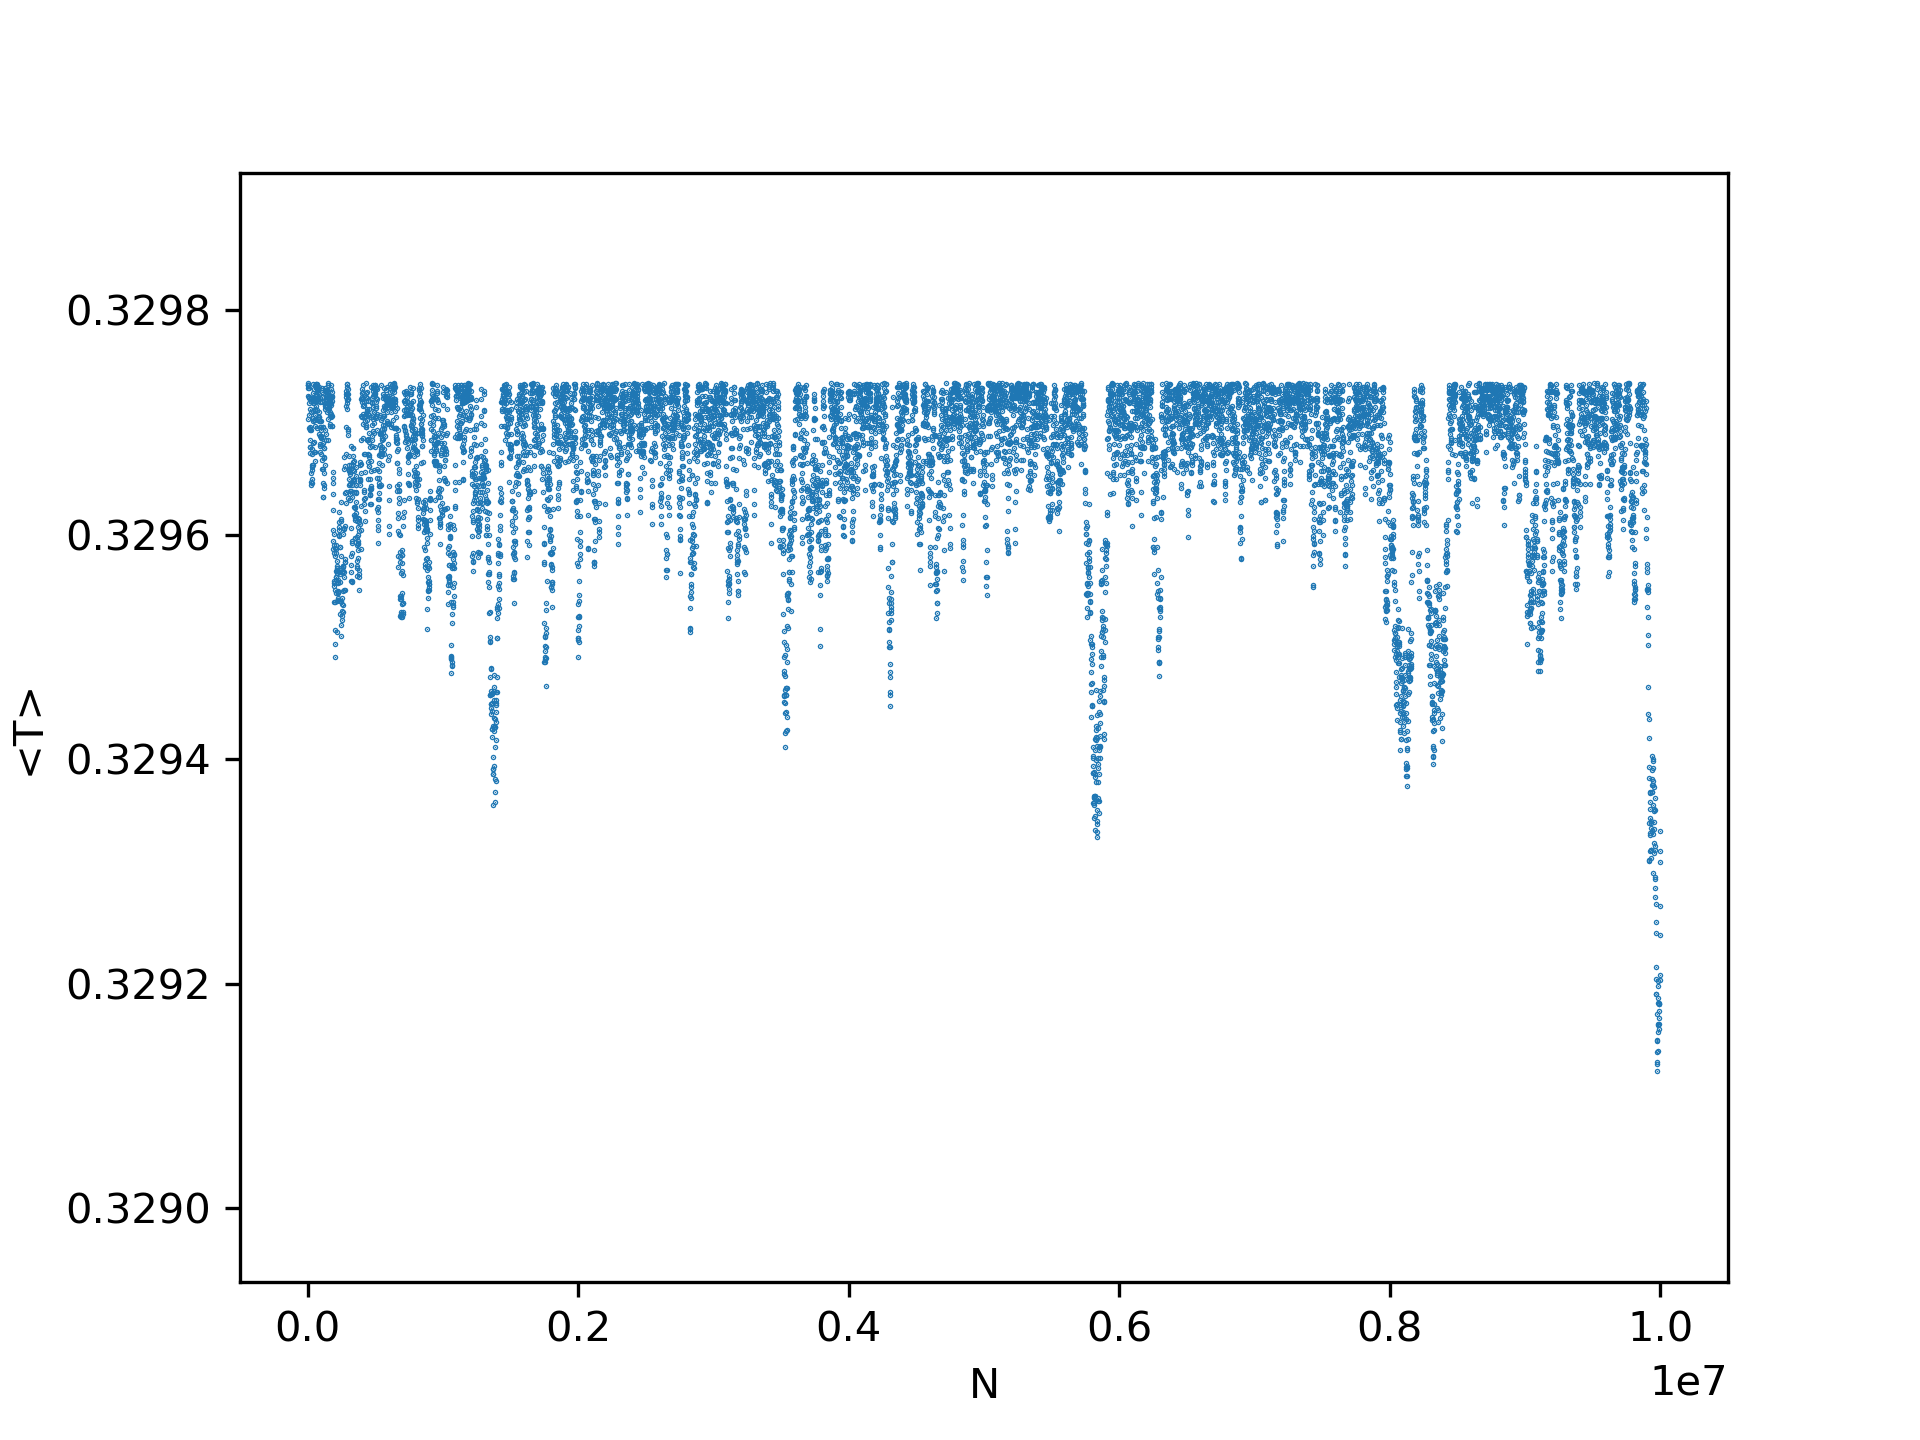
\includegraphics[bb= 0 0 460.8 345.6,width=7cm] {0.01-104-107-T.png}
}
\subfigure[$E_{d}$统计结果]{
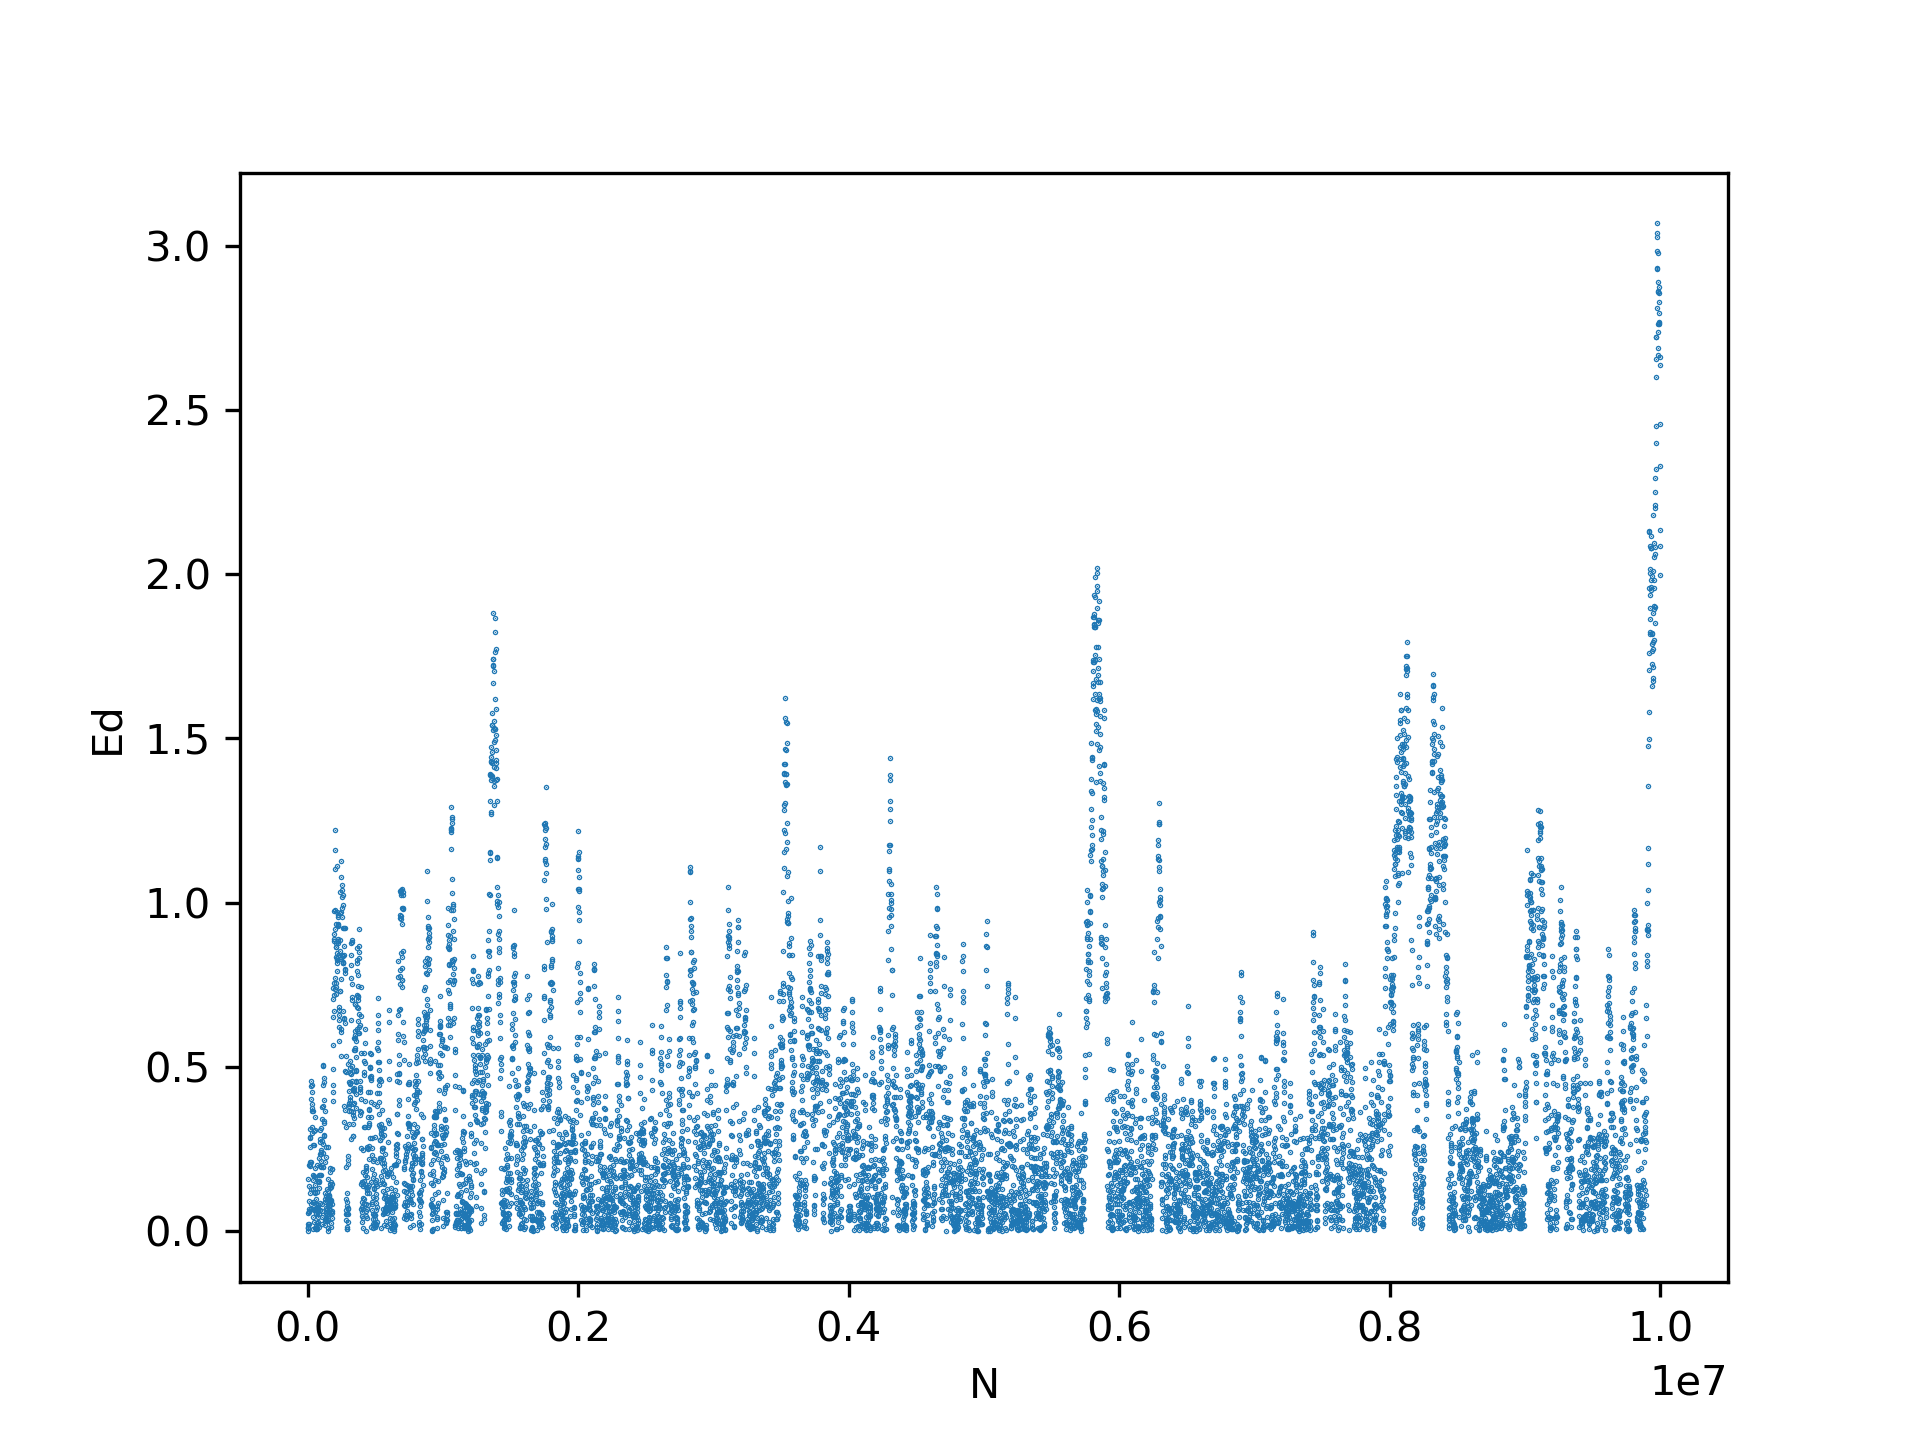
\includegraphics[bb= 0 0 460.8 345.6,width=7cm] {0.01-104-107-Ed.png}
}       
\subfigure[粒子速度$v$的最终分布]{
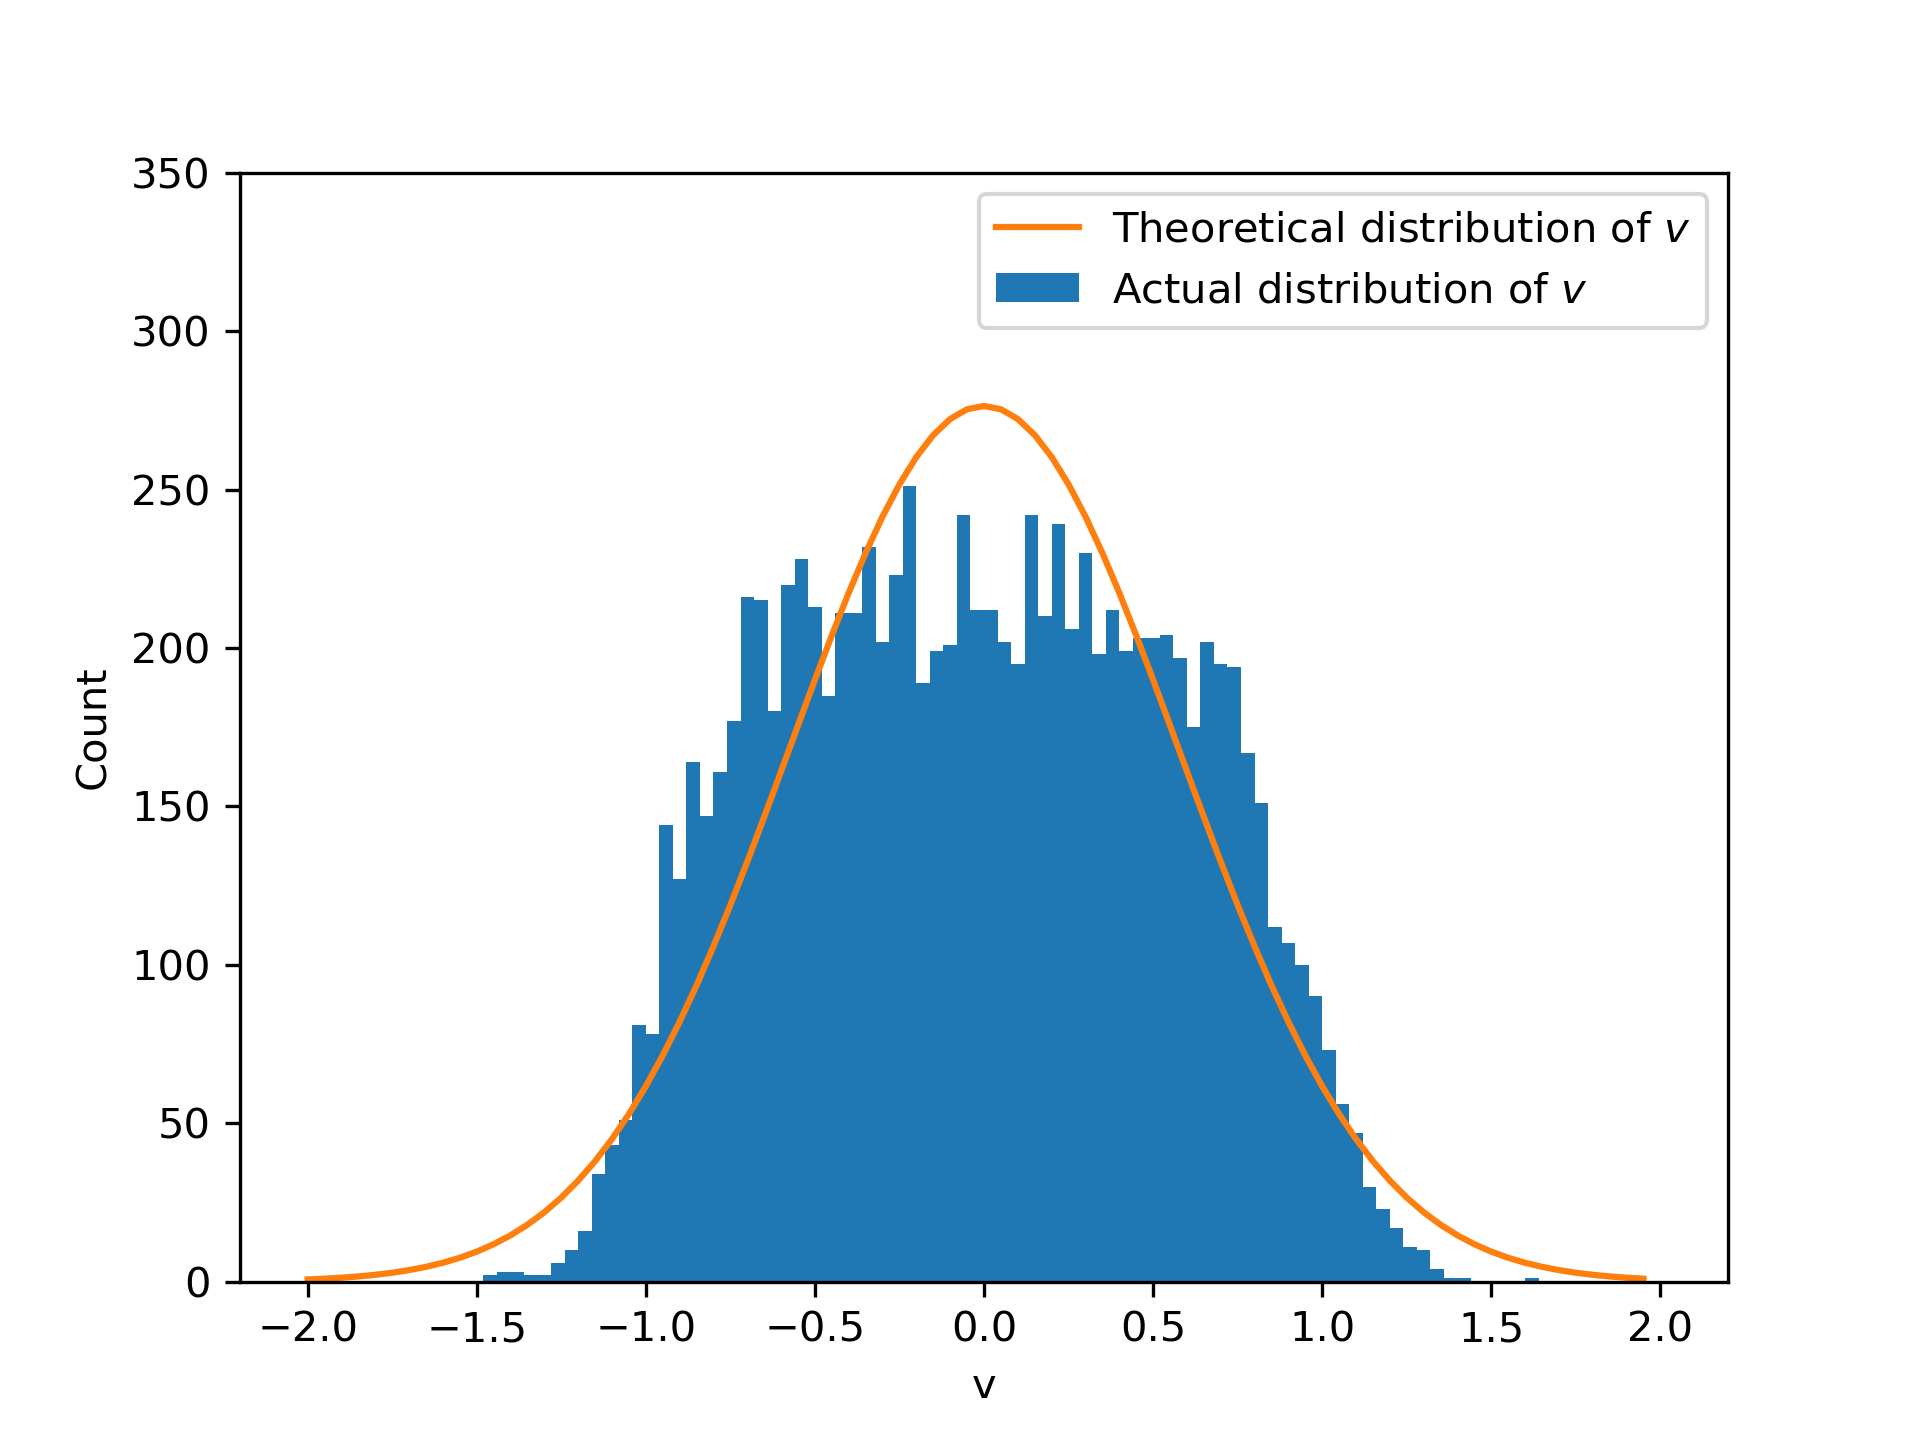
\includegraphics[bb= 0 0 460.8 345.6,width=7cm] {0.01-104-107-v.png}
}   
\subfigure[$E_{d}$的分布]{
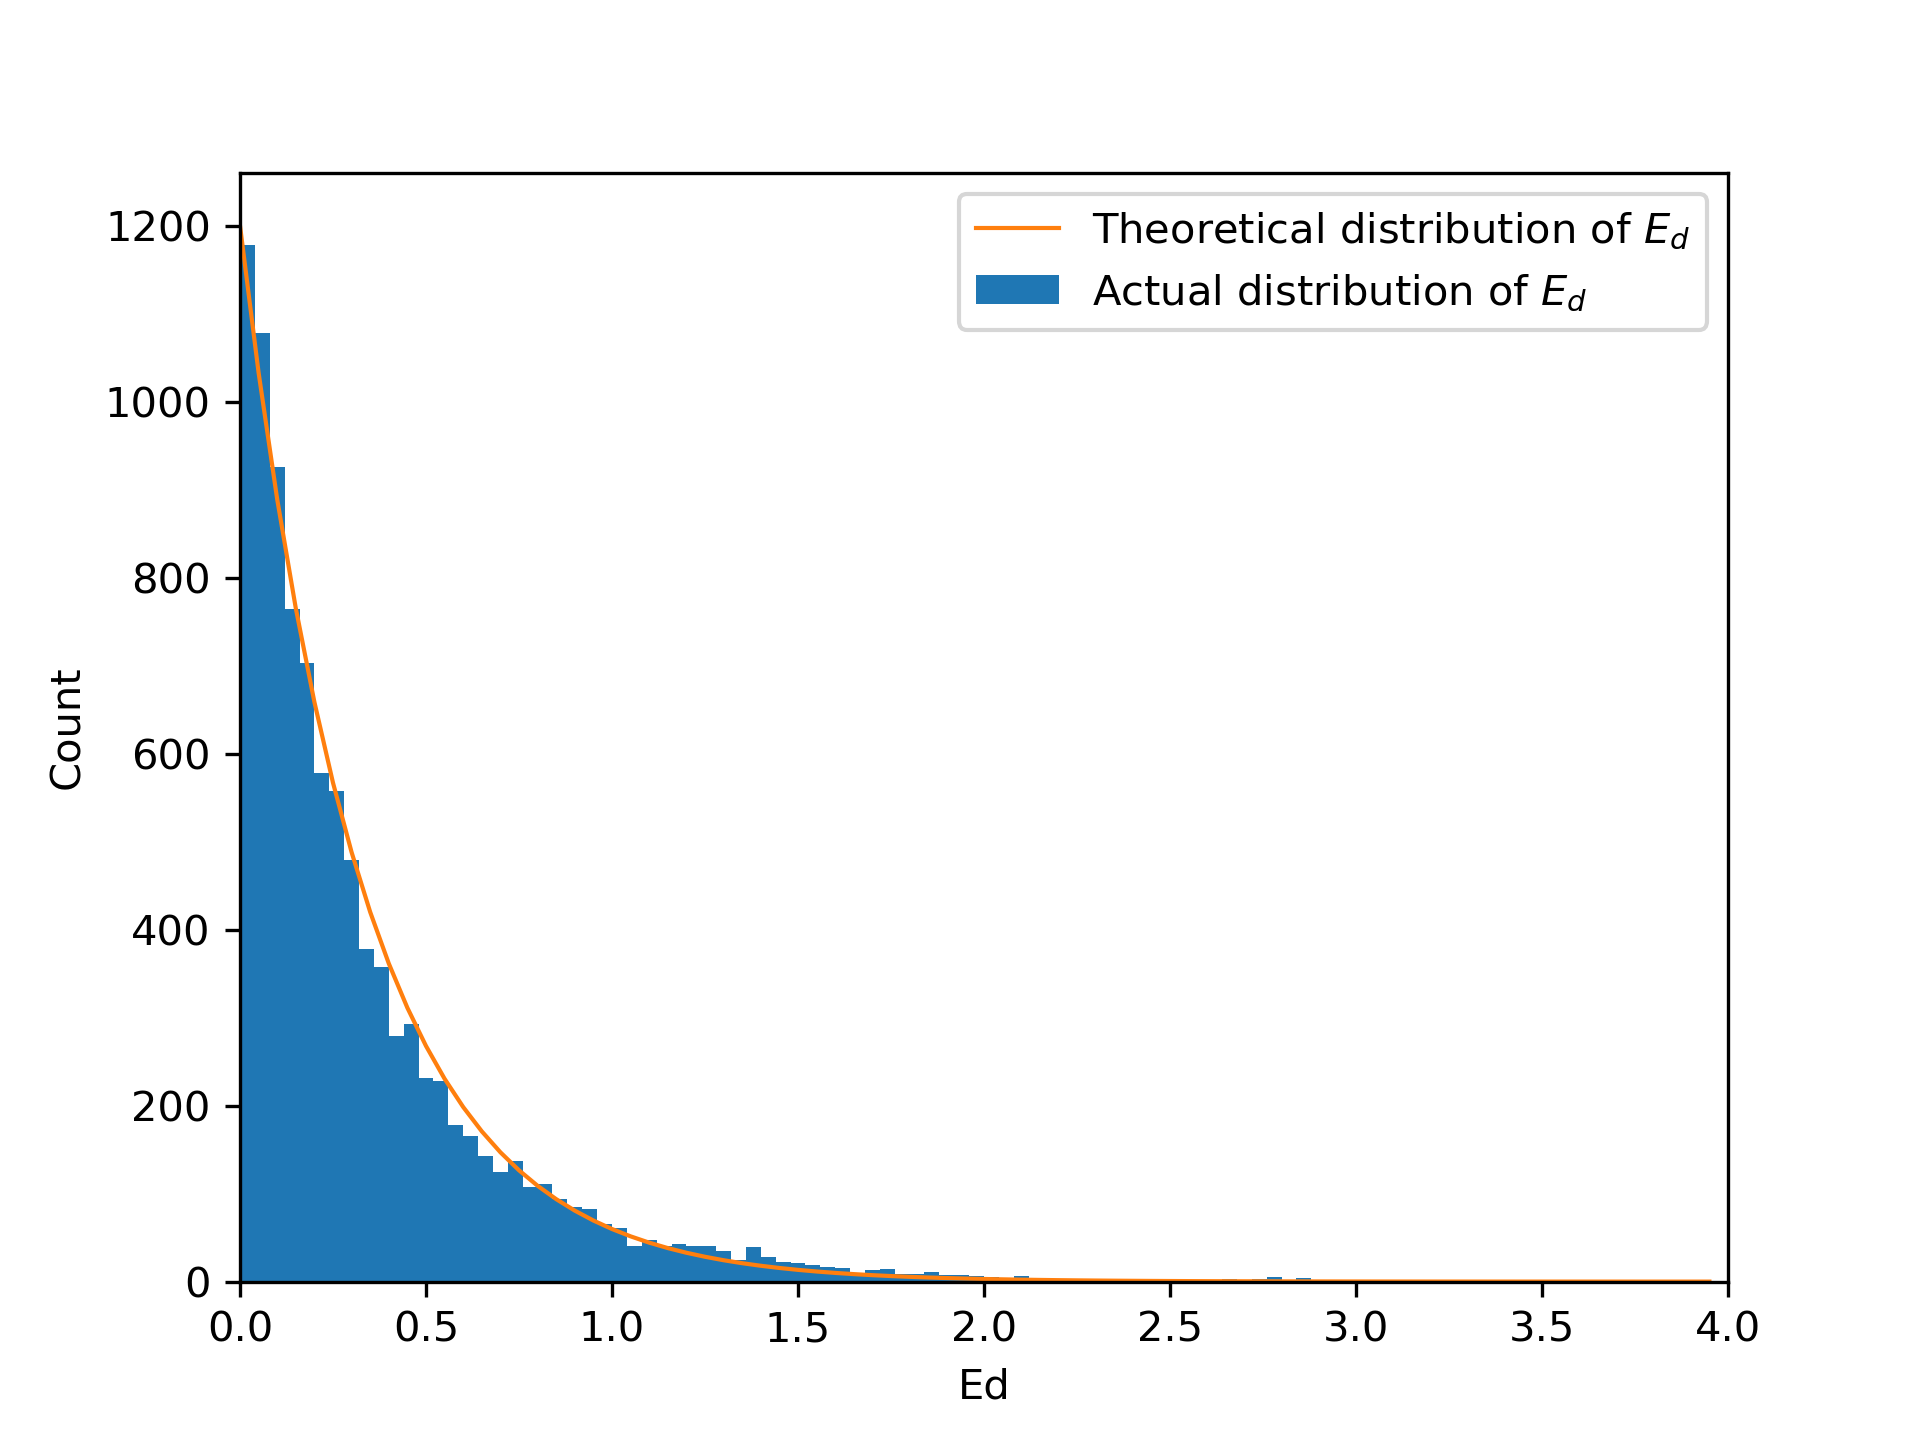
\includegraphics[bb= 0 0 460.8 345.6,width=7cm] {0.01-104-107-Ed-2.png}
}                             
\caption{$\Delta = 0.01$,$n=10^{4}$,$N=10^{7}$,每计算$1000$步统计$T,E_{d}$的结果}      
\end{figure}

可以看出,当$\Delta$减小时,确实使$E_{d}$更加接近理论分布,但是与此同时,在相同总模拟步数下,由于步数的减小,导致在此步数下系统并未达到平衡态,导致$v$的分布偏离平衡时的理论分布。

所以为了模拟的更加真实性,速度改变步长的设定既不能太小,也不能太大。

值得注意的是,从$E_{d}$的统计结果来看,发现此时每一步间的关联性比较大,出现多出类似尖峰状的形状,表明在某一步数区间内,$E_{d}$随步数增加而增加,某一区间内随步数增加而减小。这也就意味着在某些步数区间内,系统能量的该变量$\Delta E$都为负值而在另外一些区间内,都为正值。对于这样的现象,本人没有想到合理的令人满意的解释,可能由于随机数的产生存在某种关联性导致。
 

\newpage
\section{附录}

\begin{appendices}


\section{Metropois算法抽样C语言源程序}
\begin{lstlisting}[language = C]
#include <stdio.h>
#include <stdlib.h>
#include <time.h>
#include <math.h>
#define a 16807
#define b 0
#define m 2147483647
#define r (m%a)
#define q (m/a)


//写文件子程序,输入写成文件名称字符串str,数据来源于数组num,数据总数n
int my_filewriter(char str[],double num[],int n){
    FILE * fp;
    fp = fopen(str,"w+");

    for(int i=0;i<(n-1);i++)
    {
        fprintf(fp,"%lf,",num[i]);

    }
    fprintf(fp,"%lf",num[n-1]);    //最后一个数据后不加 ","
    fclose(fp);
    return 0;
}



int main(int argc, const char * argv[]) {
    time_t t;
    srand((unsigned) time(&t));  //给随机函数赋种子值
    int n = 10000;    //一维粒子的总个数
    double *v = malloc(sizeof(double)*n);   //一维粒子的速度数组
    double dE;   //能量差
    double dv;  //某一步对某一粒子速度的改变量
    double delta = 0.1; //每一步每一粒子速度的改变范围在[-delta,delat]之间
    int N = 10000000;   //总步数
    int i;   //粒子的标号
    int flag = 0;
    int flag2 = 0;
    int step = 1000;  //计算粒子平均温度与Ed的步数间隔
    
    double *T = malloc(sizeof(double)*N/step + 1);   //不同步数的一维粒子温度
    double *Td = malloc(sizeof(double)*N/step + 1);  //不同步数的demon能
    double Ed = 0;   //demon能初值为0
 
    for(int j =0;j<N/step;j++){
        T[j] = 0;
    }
    
    for(int j = 0;j<n;j++){
        v[j] = 2*(double)rand()/RAND_MAX - 1;   //粒子速度初始化
    }
    
    
    for(int k = 0;k<n;k++){  //计算模拟后的系统平均温度
        T[0] += pow( v[k],2 )/n;
    }
    Td[0] = 0;
    flag++;
    
    
    for(int j = 0;j<N;){
        i = rand() % n;
        dv = 2*delta*rand()/(double)RAND_MAX-delta;
           
        dE = 0.5*( pow(v[i]+dv,2)-pow(v[i],2) );
        if(dE<0){
            v[i] += dv;
            Ed -= dE;
            j++;
        }
        else{
            if(Ed >= dE){
                v[i] += dv;
                Ed -= dE;
                j++;
            }
        }
        if(j % step == 0 && j != 0 && j!= flag2){  //当步数差了step步时计算T,flag2为判断是否与上步相同的标志
            flag2 = j;
            for(int k = 0;k<n;k++){  //计算模拟后的系统平均温度
                T[flag] += pow( v[k],2 )/n;
            }
            Td[flag] = Ed;
            flag++;
        }
    }
    
    my_filewriter("v.dat", v, n);
    my_filewriter("T.dat", T, N/step + 1);
    my_filewriter("Ed.dat", Td, N/step + 1);
    
    return 0;
}

\end{lstlisting}

\newpage

\section{可视化绘图及数据处理Python程序源码}
\begin{lstlisting}[language = python]
import matplotlib.pyplot as plt
import numpy as np
import math

plt.rcParams['savefig.dpi'] = 300 #图片像素
plt.rcParams['figure.dpi'] = 300 #分辨率
# 默认的像素:[6.0,4.0],分辨率为100,图片尺寸为 600&400
fig1 = plt.figure()
fig2 = plt.figure()
fig3 = plt.figure()
fig4 = plt.figure()

ax1 = fig1.add_subplot(111)
ax2 = fig2.add_subplot(111)
ax3 = fig3.add_subplot(111)
ax4 = fig4.add_subplot(111)

v = []
T = []
vcul = []
Ed = []
Edcul = []
XT = []
delta = 0.1
n = 4
N = 7
step = 1000

XT = np.arange(0, 10**N + step/2, step)

with open('problem 17/v.dat', 'r') as f:
    while True:
        lines = f.readline() # 整行读取数据
        if not lines:
            break
        v = [float(i) for i in lines.split(',')]  # 将整行数据分割处理
    v = np.array(v) # 将数据从list类型转换为array类型。


with open('problem 17/T.dat', 'r') as f:
    while True:
        lines = f.readline() # 整行读取数据
        if not lines:
            break
        T = [float(i) for i in lines.split(',')]  # 将整行数据分割处理
    T = np.array(T) # 将数据从list类型转换为array类型。

with open('problem 17/Ed.dat', 'r') as f:
    while True:
        lines = f.readline() # 整行读取数据
        if not lines:
            break
        Ed = [float(i) for i in lines.split(',')]  # 将整行数据分割处理
    Ed = np.array(Ed) # 将数据从list类型转换为array类型。


vcul = (10**n)*0.04*math.sqrt(3/(2*math.pi))*np.exp(-3*np.power(np.arange(-2, 2, 0.05), 2)/2)
Edcul = (10**N/step)*0.04*np.exp(-3*np.arange(0, 4, 0.05))*3


ax1.hist(v, np.arange(-2, 2 + 0.04/2, 0.04), label=r'Actual distribution of $v$')  # DLA模拟结果散点图
ax1.plot(np.arange(-2, 2, 0.05), vcul, label=r'Theoretical distribution of $v$')
ax1.set_xlabel('v')
ax1.set_ylabel('Count')
ax1.legend(loc=1)
ax1.set_ylim(0, 350)
#ax1.set_aspect('equal')
fig1.savefig(str(delta)+'-10'+str(n)+'-10'+str(N)+'-v.png')

ax2.scatter(XT, T, s=0.1)
ax2.set_xlabel('N')
ax2.set_ylabel('<T>')
#ax2.set_aspect('equal')
fig2.savefig(str(delta)+'-10'+str(n)+'-10'+str(N)+'-T.png')


ax3.scatter(XT, Ed, s=0.1, label=r'$Ed$')
ax3.set_xlabel('N')
ax3.set_ylabel('Ed')
#ax3.set_aspect('equal')
fig3.savefig(str(delta)+'-10'+str(n)+'-10'+str(N)+'-Ed.png')

ax4.hist(Ed, np.arange(0, 4 + 0.04/2, 0.04), label=r'Actual distribution of $E_{d}$')  # DLA模拟结果散点图
ax4.plot(np.arange(0, 4, 0.05), Edcul, lw=1, label=r'Theoretical distribution of $E_{d}$')
ax4.set_xlabel('Ed')
ax4.set_ylabel('Count')
ax4.set_xlim(0, 4)
ax4.legend(loc = 1)
fig4.savefig(str(delta)+'-10'+str(n)+'-10'+str(N)+'-Ed-2.png')

\end{lstlisting}


\end{appendices}



\end{document}
